\chapter{Misturas Homogêneas de Substâncias Puras}
\label{chap:homogeneousMixtures}

    O gás natural é uma mistura homogênea de substâncias puras. Contém cerca de
    \num{50} a \SI{95}{\percent} de metano, mas também etano, propano, butano e
    outros hidrocarbonetos mais pesados. O ar puro é uma mistura de nitrogênio,
    oxigênio e argônio, também uma mistura homogênea. Misturas homogêneas de
    substâncias puras são as misturas cujas propriedades termodinâmicas são
    uniformes em toda a mistura. E a mistura de fases? Esta é heterogênea, pois
    suas propriedades (exceto a temperatura e a pressão que garantem o
    equilíbrio) não são uniformes ao longo de toda a mistura.

    Torna-se claro que se quisermos ampliar a nossa capacidade de modelar e
    resolver os problemas reais precisamos descobrir alguma maneira de obter as
    propriedades termodinâmicas das misturas homogêneas. Mas como?


    \section{O Postulado Estendido dos Estados}
    \label{sec:extendedPostulateOfStates}

    Parece um questão de bom-senso científico deduzir que o estado de uma
    mistura homogênea, ou seja, suas propriedades termodinâmicas, deve depender
    de algum modo das propriedades de seus componentes. Assim, se em uma
    mistura homogênea binária a \gls{temperature} e \gls{pressure}, isto é, com
    apenas dois componentes A e B, houver muito mais A do que B, as
    propriedades tenderão a ficar mais próximas de A e vice-versa.

    Estabeleceremos, inicialmente, que para os sistemas compostos de misturas
    homogêneas, cujo trabalho mecânico relevante for do tipo
    \gls{pressure}\diff{\gls{volume}}, além do trabalho de eixo, o estado
    intensivo da mistura será estabelecido por duas propriedades termodinâmicas
    intensivas independentes e pela composição da mistura. Esta afirmação é
    conhecida como o \emph{Postulado Estendido dos Estados} e, assim como a sua
    contrapartida para substâncias puras, é de fundamental importância para a
    solução de problemas que envolvem misturas.

    Como consequência, sabemos que qualquer propriedade termodinâmica intensiva
    de uma mistura homogênea, definida ou a definir, não passa de uma variável
    dependente, ou uma função, de \gls{pressure} e \gls{temperature} da
    mistura, se estas forem independentes, bem como da composição da mistura.


    \section{Propriedades Molares Parciais}

    Seja um sistema fechado que
    é uma mistura composta de apenas duas substâncias puras A e B, uma mistura
    binária. O número de moles de A é \propcomp{numberMoles}{A} e de B é
    \propcomp{numberMoles}{B}. As frações molares de A e B na mistura são
    respectivamente, sendo $\gls{numberMoles} = \propcomp{numberMoles}{A}
    + \propcomp{numberMoles}{B}$, o número total de moles da mistura:
    %
    \begin{equation} \label{eq:7.1}
        \propcomp{moleFraction}{A}
        =
        \frac{
            \propcomp{numberMoles}{A}
        }{
            \gls{numberMoles}
        }
        \,\,\,\,
        \text{e}
        \,\,\,\,
        \propcomp{moleFraction}{B}
        =
        \frac{
            \propcomp{numberMoles}{B}
        }{
            \gls{numberMoles}
        }\,.
    \end{equation}
    %
    Evidentemente:
    %
    \begin{equation} \label{eq:7.2}
        \propcomp{moleFraction}{A}
        +
        \propcomp{moleFraction}{B}
        =
        1\,.
    \end{equation}

    Consideremos o volume da mistura. Pelo Postulado Estendido dos Estados
    sabemos que o volume total da mistura \gls{volume} será dado por uma função
    de duas propriedades intensivas independentes, por exemplo,
    \gls{temperature}, \gls{pressure} e dos números de moles de A e de B:
    %
    \begin{equation} \label{eq:7.3}
        \gls{volume}
        =
        \gls{volume}
        \functionOf{
            \gls{temperature},
            \gls{pressure},
            \propcomp{numberMoles}{A},
            \propcomp{numberMoles}{B}
        }\,,
    \end{equation}

    e, pela regra da cadeia,
    %
    \begin{equation} \label{eq:7.4}
        \diff{\gls{volume}}
        =
        \ddxconsty{
            \gls{volume}
        }{
            \gls{temperature}
        }{
            \gls{pressure},
            \propcomp{numberMoles}{A},
            \propcomp{numberMoles}{B}
        }
        \diff{\gls{temperature}}
        +
        \ddxconsty{
            \gls{volume}
        }{
            \gls{pressure}
        }{
            \gls{temperature},
            \propcomp{numberMoles}{A},
            \propcomp{numberMoles}{B}
        }
        \diff{\gls{pressure}}
        +
        \ddxconsty{
            \gls{volume}
        }{
            \propcomp{numberMoles}{A}
        }{
            \gls{temperature},
            \gls{pressure},
            \propcomp{numberMoles}{B}
        }
        \diff{\propcomp{numberMoles}{A}}
        +
        \ddxconsty{
            \gls{volume}
        }{
            \propcomp{numberMoles}{B}
        }{
            \gls{temperature},
            \gls{pressure},
            \propcomp{numberMoles}{A}
        }
        \diff{\propcomp{numberMoles}{B}}\,.
    \end{equation}

    Se quisermos analisar o comportamento do volume total da mistura somente
    devido as alterações do número de moles, enquanto mantendo a temperatura e
    a pressão inalteradas:
    %
    \begin{equation} \label{eq:7.5}
        \diff{\gls{volume}}_{
            \gls{temperature},
            \gls{pressure}
        }
        =
        \ddxconsty{
            \gls{volume}
        }{
            \propcomp{numberMoles}{A}
        }{
            \gls{temperature},
            \gls{pressure},
            \propcomp{numberMoles}{B}
        }
        \diff{\propcomp{numberMoles}{A}}
        +
        \ddxconsty{
            \gls{volume}
        }{
            \propcomp{numberMoles}{B}
        }{
            \gls{temperature},
            \gls{pressure},
            \propcomp{numberMoles}{A}
        }
        \diff{\propcomp{numberMoles}{B}}\,.
    \end{equation}

    Tendo em vista que os coeficientes de \diff{\propcomp{numberMoles}{A}}
    e \diff{\propcomp{numberMoles}{B}} são propriedades intensivas (por
    quê?), ou seja, não se alteram com a extensão do sistema, e que as
    propriedades extensivas dependem linearmente da massa, podemos integrar a
    \cref{eq:7.5}, utilizando o Teorema de Euler das funções homogêneas,
    obtendo:
    %
    \begin{equation} \label{eq:7.6}
        \gls{volume}_{
            \gls{temperature},
            \gls{pressure}
        }
        =
        \ddxconsty{
            \gls{volume}
        }{
            \propcomp{numberMoles}{A}
        }{
            \gls{temperature},
            \gls{pressure},
            \propcomp{numberMoles}{B}
        }
        \propcomp{numberMoles}{A}
        +
        \ddxconsty{
            \gls{volume}
        }{
            \propcomp{numberMoles}{B}
        }{
            \gls{temperature},
            \gls{pressure},
            \propcomp{numberMoles}{A}
        }
        \propcomp{numberMoles}{B}\,.
    \end{equation}

    Definimos, então, \partmolalprop{volume}{i}, o volume parcial molar (ou
    molar parcial) do componente i na mistura a \gls{temperature} e
    \gls{pressure} como:
    %
    \begin{equation} \label{eq:7.7}
        \partmolalprop{volume}{i}
        \equiv
        \ddxconsty{
            \gls{volume}
        }{
            \propcomp{numberMoles}{i}
        }{
            \gls{temperature},
            \gls{pressure},
            \propcomp{numberMoles}{j \neq i}
        }\,,
        \,\,\,\,
        \forall i\,,
    \end{equation}
    %
    e substituímos os volumes parciais molares na \cref{eq:7.6}:
    %
    \begin{equation} \label{eq:7.8}
        \gls{volume}
        =
        \partmolalprop{volume}{A}
        \functionOf{
            \gls{temperature},
            \gls{pressure},
            \propcomp{moleFraction}{A}
        }
        \propcomp{numberMoles}{A}
        +
        \partmolalprop{volume}{B}
        \functionOf{
            \gls{temperature},
            \gls{pressure},
            \propcomp{moleFraction}{B}
        }
        \propcomp{numberMoles}{B}\,,
    \end{equation}
    %
    onde fica claro que os volumes parciais molares são propriedades intensivas
    e, portanto, pelo Postulado Estendido dos Estados dependem de duas
    propriedades intensivas independentes e da composição e não diretamente do
    número de moles dos componentes.

    A definição na \cref{eq:7.7} serve, na verdade, para qualquer propriedade
    extensiva \gls{thermodynamicProperty}, qualquer que seja o número de
    componentes da mistura. Assim, para \gls{numberSpecies} componentes:
    %
    \begin{equation} \label{eq:7.9}
        \gls{thermodynamicProperty}
        =
        \sum\limits_{i = 1}^{\gls{numberSpecies}}{
            \partmolalprop{thermodynamicProperty}{i}
            \functionOf{
                \gls{temperature},
                \gls{pressure},
                \propcomp{moleFraction}{j \neq i}
            }
            \propcomp{numberMoles}{i}
        }
        \,\,\,\,
        \text{e}
        \,\,\,\,
        \gls{intThermodynamicProperty}
        =
        \frac{
            \gls{thermodynamicProperty}
        }{
            \gls{numberMoles}
        }
        =
        \sum\limits_{i = 1}^{\gls{numberSpecies}}{
            \partmolalprop{thermodynamicProperty}{i}
            \functionOf{
                \gls{temperature},
                \gls{pressure},
                \propcomp{moleFraction}{j \neq i}
            }
            \propcomp{moleFraction}{i}
        }\,.
    \end{equation}

    Você poderá ter percebido de passagem que, a partir de
    %
    \begin{equation}
        \diff{\gls{thermodynamicProperty}}
        =
        \sum\limits_{i = 1}^{\gls{numberSpecies}}{
            \partmolalprop{thermodynamicProperty}{i}
            \diff{\propcomp{numberMoles}{i}}
        }\,,
    \end{equation}
    %
    e da \cref{eq:7.9}, podemos concluir que
    %
    \begin{equation} \label{eq:7.10}
        \diff{\gls{thermodynamicProperty}}
        =
        \sum\limits_{i = 1}^{\gls{numberSpecies}}{
            \propcomp{numberMoles}{i}
            \diff{\partmolalprop{thermodynamicProperty}{i}}
        }\,,
    \end{equation}
    %
    que são conhecidas como as \emph{Equações de Gibbs-Duhem}.


    \section{Mais do que Uma Questão de Nomenclatura}

    A nomenclatura pode ser bastante confusa, se não formos bem cuidadosos e
    consistentes. Então, \state{\gls{thermodynamicProperty}}{j},
    \state{\gls{intThermodynamicProperty}}{j} e
    \state{\molar{\gls{intThermodynamicProperty}}}{j} são respectivamente
    \gls{thermodynamicProperty} total, \gls{intThermodynamicProperty}
    específico e \gls{intThermodynamicProperty} específico molar da
    \emph{mistura no estado $j$};
    \state{\propcomp{thermodynamicProperty}{i}}{j},
    \state{\propcomp{intThermodynamicProperty}{i}}{j} e
    \state{\molalpropcomp{intThermodynamicProperty}{i}}{j} são respectivamente
    \gls{thermodynamicProperty} total, \gls{intThermodynamicProperty}
    específico e \gls{intThermodynamicProperty} específico molar do
    \emph{componente puro $i$ no estado $j$}. Finalmente,
    \state{\partmolalprop{thermodynamicProperty}{i}}{j} corresponde a
    \gls{thermodynamicProperty} parcial molar de $i$ na mistura no estado $j$.
    Se você tem dúvidas, experimente substituir \gls{thermodynamicProperty} por
    uma propriedade extensiva, tal como o volume... De qualquer maneira você
    não deve prosseguir sem que tenha o completo domínio dessa nomenclatura.

    Reiteramos aqui também a notação para caracterizar o estado. Assim,
    \state{\propcomp{numberMoles}{A}}{1} indica o número de moles do componente
    A no estado $1$.  Lembre-se: subscrito - componente; sobrescrito - estado.
    O que será então \state{\gls{volume}}{2}?  Isso mesmo, \emph{volume total
    da mistura} no estado 2... Note que com essas convenções no presente texto
    você nunca encontrará nenhuma propriedade
    \molar{\gls{thermodynamicProperty}}, assim sem subscrito, pois isto não tem
    significado algum.


    \section{As Misturas Homogêneas e as Relações Fundamentais}

    Como ficam as relações fundamentais para o caso das misturas homogêneas?
    Sem perda de generalidade, considere uma mistura tal que
    $\gls{internalEnergy} = \gls{internalEnergy}\functionOf{\gls{entropy},
    \gls{volume}, \propcomp{numberMoles}{A}, \propcomp{numberMoles}{B}}$.
    Então, pela regra da cadeia:
    %
    \begin{equation} \label{eq:7.11}
        \diff{\gls{internalEnergy}}
        =
        \ddxconsty{
            \gls{internalEnergy}
        }{
            \gls{entropy}
        }{
            \gls{volume},
            \propcomp{numberMoles}{A},
            \propcomp{numberMoles}{B}
        }
        \diff{\gls{entropy}}
        +
        \ddxconsty{
            \gls{internalEnergy}
        }{
            \gls{volume}
        }{
            \gls{entropy},
            \propcomp{numberMoles}{A},
            \propcomp{numberMoles}{B}
        }
        \diff{\gls{volume}}
        +
        \ddxconsty{
            \gls{internalEnergy}
        }{
            \propcomp{numberMoles}{A}
        }{
            \gls{entropy},
            \gls{volume},
            \propcomp{numberMoles}{B}
        }
        \diff{\propcomp{numberMoles}{A}}
        +
        \ddxconsty{
            \gls{internalEnergy}
        }{
            \propcomp{numberMoles}{B}
        }{
            \gls{entropy},
            \gls{volume},
            \propcomp{numberMoles}{A}
        }
        \diff{\propcomp{numberMoles}{B}}\,.
    \end{equation}

    Por outro lado,
    %
    \begin{equation} \label{eq:7.12}
        \diff{\gls{internalEnergy}}
        =
        \gls{temperature}
        \diff{\gls{entropy}}
        -
        \gls{pressure}
        \diff{\gls{volume}}
        +
        \ddxconsty{
            \gls{internalEnergy}
        }{
            \propcomp{numberMoles}{A}
        }{
            \gls{entropy},
            \gls{volume},
            \propcomp{numberMoles}{B}
        }
        \diff{\propcomp{numberMoles}{A}}
        +
        \ddxconsty{
            \gls{internalEnergy}
        }{
            \propcomp{numberMoles}{B}
        }{
            \gls{entropy},
            \gls{volume},
            \propcomp{numberMoles}{A}
        }
        \diff{\propcomp{numberMoles}{B}}\,,
    \end{equation}
    %
    onde
    %
    \begin{equation} \label{eq:7.13}
        \gls{temperature}
        =
        \ddxconsty{
            \gls{internalEnergy}
        }{
            \gls{entropy}
        }{
            \gls{volume},
            \propcomp{numberMoles}{A},
            \propcomp{numberMoles}{B}
        }
        \,\,\,\,
        \text{e}
        \,\,\,\,
        \gls{pressure}
        =
        -\ddxconsty{
            \gls{internalEnergy}
        }{
            \gls{volume}
        }{
            \gls{entropy},
            \propcomp{numberMoles}{A},
            \propcomp{numberMoles}{B}
        }\,,
    \end{equation}
    %
    nas quais \gls{temperature} e \gls{pressure} representam os potenciais para
    a variação da energia interna da mistura exclusivamente com a entropia e
    exclusivamente com o volume total, respectivamente. Podemos definir, então,
    de forma análoga
    %
    \begin{equation}
        \propcomp{chemicalPotential}{A}
        =
        \ddxconsty{
            \gls{internalEnergy}
        }{
            \propcomp{numberMoles}{A}
        }{
            \gls{entropy},
            \gls{volume},
            \propcomp{numberMoles}{B}
        }
    \end{equation}
    %
    e
    %
    \begin{equation} \label{eq:7.14}
        \propcomp{chemicalPotential}{B}
        =
        \ddxconsty{
            \gls{internalEnergy}
        }{
            \propcomp{numberMoles}{B}
        }{
            \gls{entropy},
            \gls{volume},
            \propcomp{numberMoles}{A}
        }\,,
    \end{equation}
    %
    como sendo o potencial para a variação da energia interna da mistura
    exclusivamente com \propcomp{numberMoles}{A} --- potencial químico do
    componente A --- e exclusivamente com \propcomp{numberMoles}{B} ---
    potencial químico do componente B --- na mistura de A e B. Você já deve ter
    percebido que, da mesma forma que as propriedades parciais molares, o
    potencial químico de um componente da mistura é uma propriedade
    termodinâmica intensiva da mistura (por quê?). De forma generalizada,
    podemos expressar para uma mistura homogênea de \gls{numberSpecies}
    componentes:
    %
    \begin{equation} \label{eq:7.15}
        \propcomp{chemicalPotential}{i}
        =
        \ddxconsty{
            \gls{internalEnergy}
        }{
            \propcomp{numberMoles}{i}
        }{
            \gls{entropy},
            \gls{volume},
            \propcomp{numberMoles}{j \neq i}
        }
        \,\,\,\,
        \forall i, i=1,2,\ldots,n
    \end{equation}
    %
    de forma que
    %
    \begin{equation} \label{eq:7.16}
        \diff{\gls{internalEnergy}}
        =
        \gls{temperature}
        \diff{\gls{entropy}}
        -
        \gls{pressure}
        \diff{\gls{volume}}
        +
        \sum\limits_{i=1}^{\gls{numberSpecies}}{%
            \propcomp{chemicalPotential}{i}
            \diff{\propcomp{numberMoles}{i}}
        }\,.
    \end{equation}

    Uma vez que $\gls{enthalpy} = \gls{internalEnergy} +
    \gls{pressure}\gls{volume}$, você pode mostrar que:
    %
    \begin{equation} \label{eq:7.17}
        \diff{\gls{enthalpy}}
        =
        \gls{temperature}
        \diff{\gls{entropy}}
        +
        \gls{volume}
        \diff{\gls{pressure}}
        +
        \sum\limits_{i=1}^{\gls{numberSpecies}}{%
            \propcomp{chemicalPotential}{i}
            \diff{\propcomp{numberMoles}{i}}
        }\,,
    \end{equation}
    %
    com o potencial químico de cada componente $i$ agora:
    %
    \begin{equation} \label{eq:7.18}
        \propcomp{chemicalPotential}{i}
        =
        \ddxconsty{
            \gls{enthalpy}
        }{
            \propcomp{numberMoles}{i}
        }{
            \gls{entropy},
            \gls{pressure},
            \propcomp{numberMoles}{j \neq i}
        }
        \,\,\,\,
        \forall i, i=1,2,\ldots,n\,.
    \end{equation}

    De modo análogo, $\gls{GibbsFreeEnergy} = \gls{enthalpy} -
    \gls{temperature}\gls{entropy}$ e podemos escrever:
    %
    \begin{equation} \label{eq:7.19}
        \diff{\gls{GibbsFreeEnergy}}
        =
        -\gls{entropy}
        \diff{\gls{temperature}}
        +
        \gls{volume}
        \diff{\gls{pressure}}
        +
        \sum\limits_{i=1}^{\gls{numberSpecies}}{%
            \propcomp{chemicalPotential}{i}
            \diff{\propcomp{numberMoles}{i}}
        }\,.
    \end{equation}

    Então, o potencial químico de cada componente $i$ será
    %
    \begin{equation} \label{eq:7.20}
        \propcomp{chemicalPotential}{i}
        =
        \ddxconsty{
            \gls{GibbsFreeEnergy}
        }{
            \propcomp{numberMoles}{i}
        }{
            \gls{temperature},
            \gls{pressure},
            \propcomp{numberMoles}{j \neq i}
        }
        =
        \partmolalprop{GibbsFreeEnergy}{i}\,,
        \,\,\,\,
        \forall i, i=1,2,\ldots,n\,.
    \end{equation}

    Você deve reconhecer \partmolalprop{GibbsFreeEnergy}{i} como sendo a
    definição da função de Gibbs parcial molar de $i$ na mistura a
    \gls{temperature} e \gls{pressure}. Em outras palavras, o potencial químico
    de um componente em uma mistura é exatamente o mesmo que a função de Gibbs
    parcial molar do mesmo componente naquela mistura.


    \section{A Fugacidade de Misturas Homogêneas}

    Aproveitando-nos do conceito estabelecido para substância pura, podemos
    definir a fugacidade do componente i, \molalpropcomp{fugacity}{i}, em
    uma mistura homogênea qualquer a \gls{temperature} e \gls{pressure} como:
    %
    \begin{equation} \label{eq:7.21}
        \left(
            \diff{\partmolalprop{GibbsFreeEnergy}{i}}
        \right)_{
            \gls{temperature},
            \propcomp{moleFraction}{j \neq i}
        }
        =
        \gls{universalGasConstant}
        \gls{temperature}
        \diff{
            \left(
                \ln{\molalpropcomp{fugacity}{i}}
            \right)_{
                \gls{temperature},
                \propcomp{moleFraction}{j \neq i}
            }
        }\,,
    \end{equation}
    %
    desde que
    %
    \begin{equation} \label{eq:7.22}
        \lim\limits_{\gls{pressure} \rightarrow 0}{
            \left(
                \frac{
                    \molalpropcomp{fugacity}{i}
                }{
                    \propcomp{moleFraction}{i}
                    \gls{pressure}
                }
            \right)
        }
        =
        1\,.
    \end{equation}

    Em outras palavras, se a fugacidade de $i$ puro,
    \propcomp{fugacity}{i}\functionOf{\gls{temperature}, \gls{pressure}}, tende
    à pressão \gls{pressure}, então nada mais natural que a fugacidade de $i$
    na mistura, \molalpropcomp{fugacity}{i}\functionOf{\gls{temperature},
    \gls{pressure},\propcomp{moleFraction}{j \neq i}}, tenda à pressão parcial
    de $i$ na mistura de gases perfeitos. Fique atento à nossa notação: a
    fugacidade do componente $i$ na mistura tem uma barra por cima da letra
    \gls{fugacity}, além do componente $i$ como subscrito, ao passo que a
    fugacidade do componente puro não tem a barra por cima, somente o subscrito
    de $i$ puro.


    \section{As Misturas Homogêneas Binárias e Multicomponentes}

    Pois bem, seja o sistema fechado que é a mistura binária
    de \state{\propcomp{numberMoles}{A}}{1} moles do componente A e
    \state{\propcomp{numberMoles}{B}}{1} moles do componente B.

    Como já sabemos, podemos escrever: \state{\partmolalprop{volume}{B}}{1},
    \state{\partmolalprop{volume}{A}}{1},
    \state{\partmolalprop{internalEnergy}{A}}{1},
    \state{\partmolalprop{enthalpy}{B}}{1},
    \state{\partmolalprop{entropy}{B}}{1} e assim por diante, pois cada
    propriedade extensiva tem as suas correspondentes molares parciais para
    cada componente da mistura respectivamente.

    Pela própria definição, as propriedades molares parciais se combinam da
    mesma forma que as propriedades extensivas da mistura. Assim, de
    $\gls{enthalpy} = \gls{internalEnergy} + \gls{pressure}\gls{volume}$,
    obtemos $\partmolalprop{enthalpy}{i} = \partmolalprop{internalEnergy}{i} +
    \gls{pressure}\partmolalprop{volume}{i}$ e de $\gls{GibbsFreeEnergy} =
    \gls{enthalpy} - \gls{temperature}\gls{entropy}$, obtemos
    $\partmolalprop{GibbsFreeEnergy}{i} = \partmolalprop{enthalpy}{i} -
    \gls{temperature}\partmolalprop{entropy}{i}$  para cada componente $i$ da
    mistura (consegue demonstrar?).

    Por outro lado, seja a diferença de \gls{thermodynamicProperty}, denominada
    \emph{excesso de \gls{thermodynamicProperty}},  dada por
    %
    \begin{equation} \label{eq:7.23}
        \Delta \gls{thermodynamicProperty}
        =
        \gls{thermodynamicProperty}
        -
        \left(
            \propcomp{thermodynamicProperty}{A}
            +
            \propcomp{thermodynamicProperty}{B}
        \right)
        =
        \partmolalprop{thermodynamicProperty}{A}
        \propcomp{numberMoles}{A}
        +
        \partmolalprop{thermodynamicProperty}{B}
        \propcomp{numberMoles}{B}
        -
        \left(
            \molalpropcomp{intThermodynamicProperty}{A}
            \propcomp{numberMoles}{A}
            +
            \molalpropcomp{intThermodynamicProperty}{B}
            \propcomp{numberMoles}{B}
        \right)\,,
    \end{equation}
    %
    ou
    %
    \begin{equation} \label{eq:7.24}
        \Delta \gls{thermodynamicProperty}
        =
        \left(
            \partmolalprop{thermodynamicProperty}{A}
            -
            \molalpropcomp{intThermodynamicProperty}{A}
        \right)
        \propcomp{numberMoles}{A}
        +
        \left(
            \partmolalprop{thermodynamicProperty}{B}
            -
            \molalpropcomp{intThermodynamicProperty}{B}
        \right)
        \propcomp{numberMoles}{B}\,.
    \end{equation}

    % Confirmar com PRof. Woiski: é mesmo a 7.12 aqui?
    Lembre-se que \gls{thermodynamicProperty} pode ser qualquer propriedade
    extensiva. Vamos então utilizar o volume \gls{volume}. A \cref{eq:7.12}
    afirma que quando eu misturo \propcomp{numberMoles}{A} moles da substância
    pura A à temperatura \gls{temperature} e pressão \gls{pressure} e ocupando
    o volume \propcomp{volume}{A}, com \propcomp{numberMoles}{B} moles de B à
    temperatura \gls{temperature} e pressão \gls{pressure} e ocupando o volume
    \propcomp{volume}{B}, então o volume final da mistura \gls{volume} a
    \gls{temperature} e \gls{pressure} será maior ou menor do que
    $\propcomp{volume}{A} + \propcomp{volume}{B}$ pela quantidade dada pela
    \cref{eq:7.12}. Em outras palavras, para que o sistema a \gls{temperature}
    e \gls{pressure} conserve volume ao misturar A e B, ambos a
    \gls{temperature} e \gls{pressure}, cada um dos \partmolalprop{volume}{i}
    tem que ser igual a \molalpropcomp{specificVolume}{i}, isto para todo $i$.

    Voltemos ao volume de uma mistura homogênea qualquer a dois componentes.
    Sabemos, que  $\molar{\gls{specificVolume}} =
    \molar{\gls{specificVolume}}\functionOf{\gls{temperature}, \gls{pressure},
    \propcomp{moleFraction}{A}}$. Você saberia dizer por que
    \propcomp{moleFraction}{B} não aparece nesta relação funcional? Da
    \cref{eq:7.9} escrevemos
    %
    \begin{equation} \label{eq:7.25}
        \begin{aligned}
        \molar{\gls{specificVolume}}
        &=
        \partmolalprop{volume}{A}
        \propcomp{moleFraction}{A}
        +
        \partmolalprop{volume}{B}
        \propcomp{moleFraction}{B}
        =
        \partmolalprop{volume}{A}
        \propcomp{moleFraction}{A}
        +
        \partmolalprop{volume}{B}
        \left(
            1 - \propcomp{moleFraction}{A}
        \right) \\
        &=
        \left(
            \partmolalprop{volume}{A}
            -
            \partmolalprop{volume}{B}
        \right)
        \propcomp{moleFraction}{A}
        +
        \partmolalprop{volume}{B} \\
        &=
        \left(
            \partmolalprop{volume}{B}
            -
            \partmolalprop{volume}{A}
        \right)
        \left(
            1 - \propcomp{moleFraction}{A}
        \right)
        +
        \partmolalprop{volume}{A}\,.
        \end{aligned}
    \end{equation}

    Derivando em relação a \propcomp{moleFraction}{A}, enquanto mantemos
    \gls{temperature}, \gls{pressure} constantes:
    %
    \begin{equation} \label{eq:7.26}
        \DDx{
            \molar{\gls{specificVolume}}
        }{
            \propcomp{moleFraction}{A}
        }
        =
        \partmolalprop{volume}{A}
        -
        \partmolalprop{volume}{B}\,,
    \end{equation}
    %
    e, então,
    %
    \begin{equation} \label{eq:7.27}
        \molar{\gls{specificVolume}}
        =
        \DDx{
            \molar{\gls{specificVolume}}
        }{
            \propcomp{moleFraction}{A}
        }
        \propcomp{moleFraction}{A}
        +
        \partmolalprop{volume}{B}
        =
        \DDx{
            \molar{\gls{specificVolume}}
        }{
            \propcomp{moleFraction}{A}
        }
        \left(
            1 - \propcomp{moleFraction}{A}
        \right)
        +
        \partmolalprop{volume}{A}\,.
    \end{equation}

    Estas duas equações representam uma mesma reta tendo por inclinação o valor
    da derivada de \molar{\gls{specificVolume}} em \propcomp{moleFraction}{A} e
    cuja interseção em $\propcomp{moleFraction}{A} = 0$ é
    \partmolalprop{volume}{B} e em $\propcomp{moleFraction}{A} = 1$ corresponde
    a \partmolalprop{volume}{A}.

    Veja esses resultados sumarizados no diagrama da
    \cref{fig:mixtureVolumeVsMoleFraction}, que nos mostra a variação de
    \molar{\gls{specificVolume}} com \propcomp{moleFraction}{A}, mantendo-se
    \gls{temperature} e \gls{pressure} constantes. Aproveite a oportunidade e
    fixe a nomenclatura utilizada.

    \begin{figure}[!htb]
        \caption{%
            Variação do volume específico com a fração molar de A na mistura
            binária.
        }

        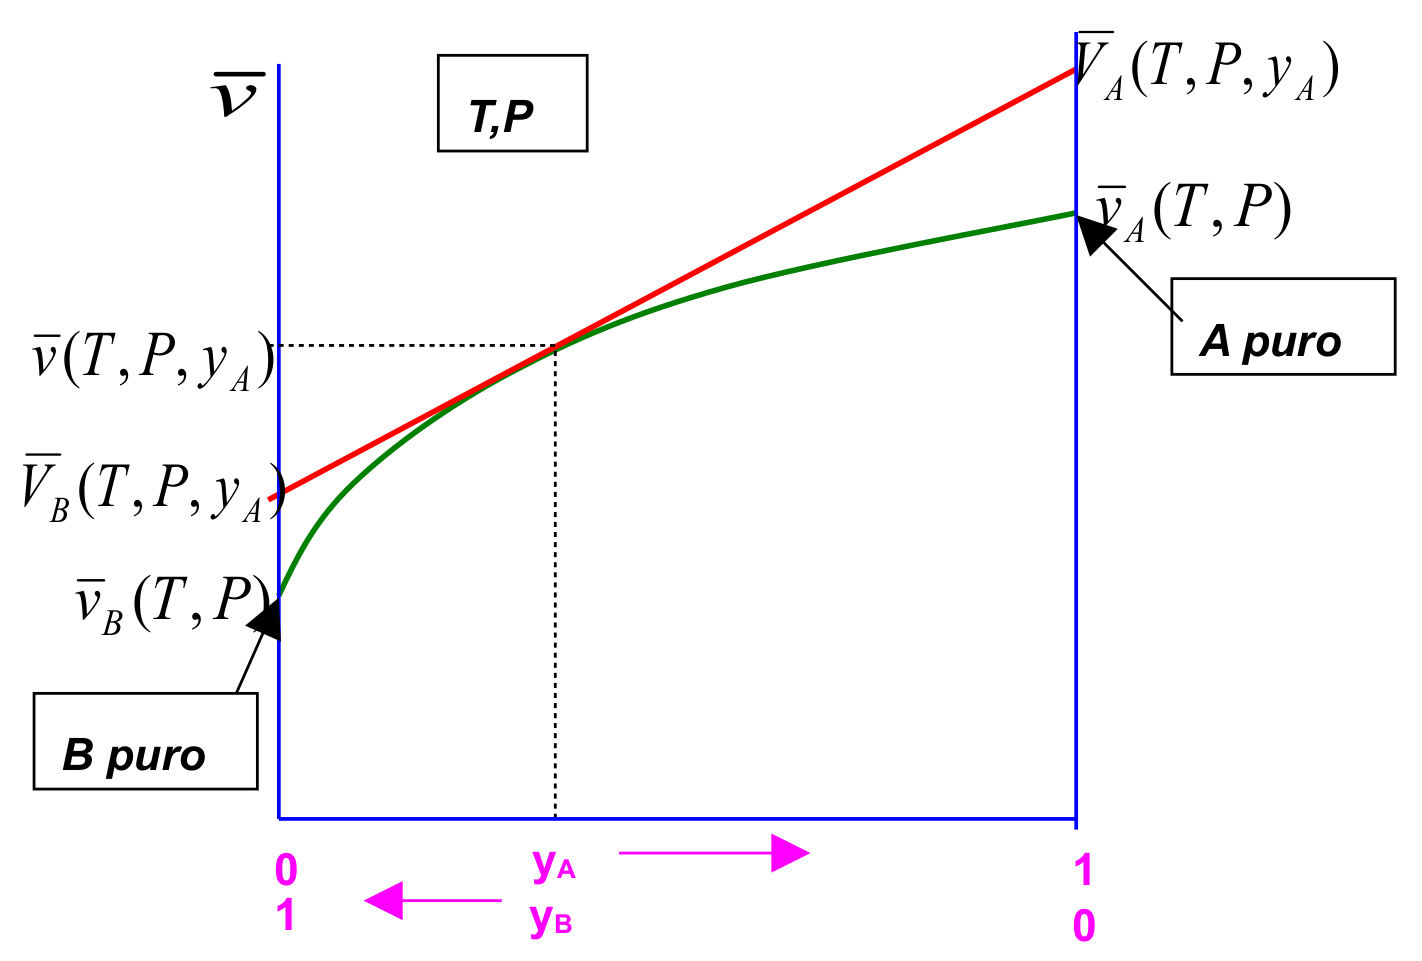
\includegraphics[
            width=0.75\textwidth
        ]   {mixtureVolumeVsMoleFraction.png}

        \label{fig:mixtureVolumeVsMoleFraction}
    \end{figure}

    Utilizamos uma mistura binária porque seu estado é definido por apenas três
    propriedades independentes (por quê?). Se fixarmos \gls{temperature},
    \gls{pressure} então resta apenas uma variável independente (qual?) e a
    produção do gráfico no plano torna-se possível. Entretanto, todas as
    definições e relações anteriores se aplicam, com alterações óbvias, a
    misturas multicomponentes, mas as curvas se tornam hiper-superfícies e as
    tangentes, hiperplanos tangentes.


    \section{As Soluções Ideais}

    As misturas homogêneas multicomponentes especiais que conservam o volume,
    ou seja, nas quais o excesso de volume $\Delta \gls{volume} = 0$, são
    denominadas \emph{soluções ideais}.

    Observando a \cref{fig:mixtureVolumeVsMoleFraction}, o que você pode dizer
    a respeito da mistura nestas condições de \gls{temperature},\gls{pressure}:
    Trata-se de uma solução ideal? O excesso de volume é positivo ou negativo
    em relação a A e B puros? Em sua opinião, qual é a curvatura de uma solução
    ideal?

    Pode-se demonstrar que se a solução for ideal, isto é, se $\Delta
    \gls{volume} = 0$:
    %
    \begin{equation} \label{eq:7.28}
        \Delta \gls{enthalpy}
        =
        \Delta \gls{internalEnergy}
        =
        0\,,
    \end{equation}
    %
    e, portanto, para cada componente $i$ da mistura a
    \gls{temperature}, \gls{pressure}, para todo $i$:
    %
    \begin{equation} \label{eq:7.29}
        \partmolalprop{enthalpy}{i}
        \functionOf{
            \gls{temperature},
            \gls{pressure},
            \propcomp{moleFraction}{j \neq i}
        }
        =
        \molalpropcomp{intEnthalpy}{i}
        \functionOf{
            \gls{temperature},
            \gls{pressure}
        }
        \,\,\,\,
        \text{e}
        \,\,\,\,
        \partmolalprop{internalEnergy}{i}
        \functionOf{
            \gls{temperature},
            \gls{pressure},
            \propcomp{moleFraction}{j \neq i}
        }
        =
        \molalpropcomp{intInternalEnergy}{i}
        \functionOf{
            \gls{temperature},
            \gls{pressure}
        }\,.
    \end{equation}

    As relações da \cref{eq:7.29} são extremamente importantes por causa de
    suas implicações, como veremos em detalhes. Então, para uma solução ideal a
    $\functionOf{\gls{temperature}, \gls{pressure}, \propcomp{moleFraction}{j
    \neq i}}$, podemos substituir o volume, a entalpia e a energia interna
    parcial molar de cada componente $i$ da mistura pelo correspondente volume,
    entalpia (e energia interna) específicos molares do mesmo componente puro
    $i$ calculados a \gls{temperature}, \gls{pressure}.

    Sabemos como ficam o volume, a energia interna e a entalpia de uma solução
    ideal. Entretanto, como fica a entropia? Pode-se também demonstrar que,
    para uma solução ideal

    \begin{equation} \label{eq:7.30}
        \Delta \gls{entropy}
        =
        -\gls{universalGasConstant}
        \sum\limits_{\gls{numberSpecies}}{
            \propcomp{numberMoles}{i}
            \ln{\propcomp{moleFraction}{i}}
        }\,,
    \end{equation}
    %
    ou seja, mesmo para soluções ideais, o excesso de entropia $\Delta
    \gls{entropy}$ não é
    nulo! A entropia parcial molar se torna então, para cada componente $i$:

    \begin{equation} \label{eq:7.31}
        \partmolalprop{entropy}{i}
        =
        \molalpropcomp{intEntropy}{i}
        \functionOf{
            \gls{temperature},
            \gls{pressure}
        }
        -
        \gls{universalGasConstant}
        \ln{\propcomp{moleFraction}{i}}\,.
    \end{equation}

    Como ficaria a função de Gibbs parcial molar cada componente da mistura em
    relação à sua respectiva função de Gibbs do componente puro a
    \gls{temperature}, \gls{pressure}?

    Uma vez que nós já aprendemos nos capítulos anteriores como determinar as
    propriedades de substâncias puras, pelo menos o problema das misturas
    modeladas como soluções ideais parece-nos completamente resolvido, não
    acha?


    \section{Retomando o Exemplo}

    Lembra-se do exemplo clássico da mistura de um gás A originalmente no
    estado 1 com o gás B originalmente no estado 2 através de uma expansão não
    resistida, esquematizado novamente na
    \cref{fig:nonResistedExpansionMixtureChap}? Vamos agora assumir que no
    recipiente rígido e adiabático, estão inicialmente
    \propcomp{numberMoles}{A} moles de A à temperatura
    \state{\propcomp{temperature}{A}}{1} e pressão
    \state{\propcomp{pressure}{A}}{1}, separados por uma membrana também rígida
    e adiabática de \propcomp{numberMoles}{B} moles de B à temperatura
    \state{\propcomp{temperature}{B}}{1} e pressão
    \state{\propcomp{pressure}{B}}{1}.

    \begin{figure}[!htb]
        \caption{%
            Exemplo de expansão não-resistida.
            binária.
        }

        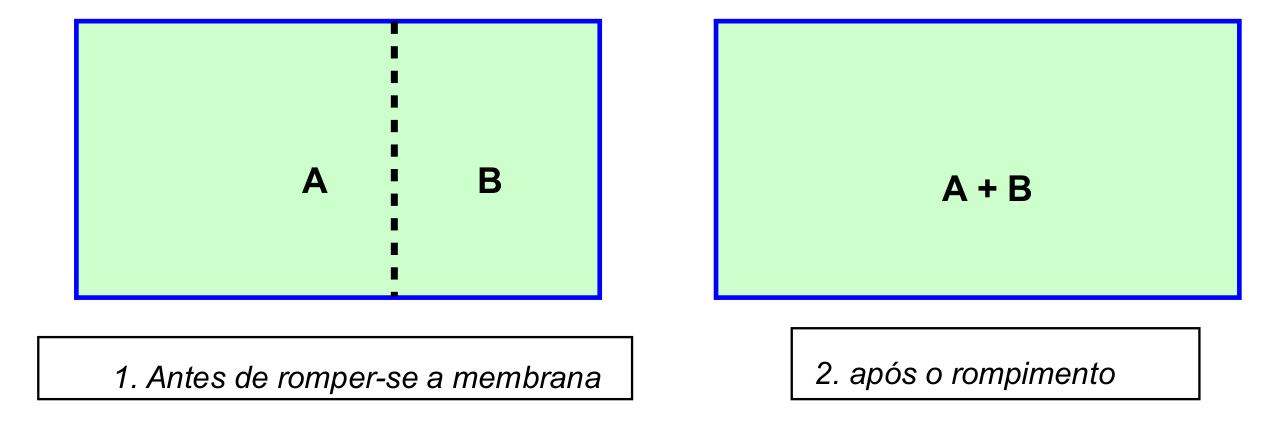
\includegraphics[
            width=0.75\textwidth
        ]   {nonResistedExpansion.png}

        \label{fig:nonResistedExpansionMixtureChap}
    \end{figure}

    Em um dado momento, rompe-se a membrana e permite-se que a pressão e a
    temperatura se equalizem nos valores de \state{\gls{temperature}}{2} e
    \state{\gls{pressure}}{2}.  O sistema é composto inicialmente de dois
    subsistemas: o subsistema gás A e o subsistema gás B.  Não há trabalho, nem
    calor, portanto o sistema está isolado.

    Da mesma forma que antes, por causa da Primeira Lei,
    %
    \begin{equation} \label{eq:7.32}
        \state{\gls{internalEnergy}}{1}
        -
        \state{\gls{internalEnergy}}{2}
        =
        0\,.
    \end{equation}
    %
    A Segunda Lei será:

    \begin{equation} \label{eq:7.33}
        \state{\gls{entropy}}{2}
        -
        \state{\gls{entropy}}{1}
        =
        \fprocess{entropyCreated}{1}{2}
        \ge
        0\,.
    \end{equation}

    Estando os fluidos A e B separados no estado 1:
    %
    \begin{equation} \label{eq:7.34}
        \state{\gls{internalEnergy}}{1}
        =
        \propcomp{numberMoles}{A}
        \state{\molalpropcomp{intInternalEnergy}{A}}{1}
        \functionOf{
            \propcomp{temperature}{A},
            \propcomp{pressure}{A}
        }
        +
        \propcomp{numberMoles}{B}
        \state{\molalpropcomp{intInternalEnergy}{B}}{1}
        \functionOf{
            \propcomp{temperature}{B},
            \propcomp{pressure}{B}
        }\,,
    \end{equation}
    %
    e tornando-se uma mistura homogênea de A e B no estado 2:
    %
    \begin{equation} \label{eq:7.35}
        \state{\gls{internalEnergy}}{2}
        \functionOf{
            \state{\gls{temperature}}{2},
            \state{\gls{pressure}}{2},
            \propcomp{numberMoles}{A},
            \propcomp{numberMoles}{B}
        }
        =
        \state{\partmolalprop{internalEnergy}{A}}{2}
        \functionOf{
            \state{\gls{temperature}}{2},
            \state{\gls{pressure}}{2},
            \state{\propcomp{moleFraction}{A}}{2}
        }
        \propcomp{numberMoles}{A}
        +
        \state{\partmolalprop{internalEnergy}{B}}{2}
        \functionOf{
            \state{\gls{temperature}}{2},
            \state{\gls{pressure}}{2},
            \state{\propcomp{numberMoles}{A}}{2}
        }
        \propcomp{numberMoles}{B}\,.
    \end{equation}

    Observe que conhecemos tudo do estado 1, pois as propriedades
    \state{\propcomp{temperature}{A}}{1}, \state{\propcomp{pressure}{A}}{1},
    \state{\propcomp{temperature}{B}}{1}, \state{\propcomp{pressure}{B}}{1},
    \propcomp{numberMoles}{A} e \propcomp{numberMoles}{B} estão definidas para
    cada um dos subsistemas. Entretanto, não sabemos de maneira geral como
    determinar as propriedades parciais molares. Para avançar na solução,
    precisamos de um modelo para a mistura do estado 2. Vamos então admitir que
    ela se comporta como uma \emph{solução ideal}. Dessa forma,
    %
    \begin{equation} \label{eq:7.36}
        \begin{aligned}
        \propcomp{numberMoles}{A}
        \state{\molalpropcomp{intInternalEnergy}{A}}{1}
        \functionOf{
            \state{\propcomp{temperature}{A}}{1},
            \state{\propcomp{pressure}{A}}{1}
        }
        +
        \propcomp{numberMoles}{B}
        \state{\molalpropcomp{intInternalEnergy}{B}}{1}
        \functionOf{
            \state{\propcomp{temperature}{B}}{1},
            \state{\propcomp{pressure}{B}}{1}
        }
        &=
        \propcomp{numberMoles}{A}
        \state{\molalpropcomp{intInternalEnergy}{A}}{2}
        \functionOf{
            \state{\gls{temperature}}{2},
            \state{\gls{pressure}}{2}
        }\\
        &+
        \propcomp{numberMoles}{B}
        \state{\molalpropcomp{intInternalEnergy}{B}}{2}
        \functionOf{
            \state{\propcomp{temperature}{B}}{2},
            \state{\propcomp{pressure}{B}}{2}
        }\,.
        \end{aligned}
    \end{equation}

    Por causa da necessária independência das bases, todos os problemas podem e
    devem ser equacionados como diferenças de propriedades termodinâmicas.
    Neste caso,
    %
    \begin{equation} \label{eq:7.37}
        \begin{aligned}
        &\propcomp{numberMoles}{A}
        \left[
            \state{\molalpropcomp{intInternalEnergy}{A}}{1}
            \functionOf{
                \state{\propcomp{temperature}{A}}{1},
                \state{\propcomp{pressure}{A}}{1}
            }
            -
            \state{\molalpropcomp{intInternalEnergy}{A}}{2}
            \functionOf{
                \state{\gls{temperature}}{2},
                \state{\gls{pressure}}{2}
            }
        \right]
        +\\
        +&
        \propcomp{numberMoles}{B}
        \left[
            \state{\molalpropcomp{intInternalEnergy}{B}}{1}
            \functionOf{
                \state{\propcomp{temperature}{B}}{1},
                \state{\propcomp{pressure}{B}}{1}
            }
            -
            \state{\molalpropcomp{intInternalEnergy}{B}}{2}
            \functionOf{
                \state{\gls{temperature}}{2},
                \state{\gls{pressure}}{2}
            }
        \right]
        =
        0\,.\\
        \end{aligned}
    \end{equation}
    %
    na forma de diferenças de energia interna de substâncias puras. Observe
    que nós estamos com apenas uma equação e duas incógnitas
    $(\state{\gls{temperature}}{2}, \state{\gls{pressure}}{2}$. Precisamos de
    mais uma equação. Esta surgirá da hipótese que o recipiente é rígido e,
    portanto
    %
    \begin{equation} \label{eq:7.38}
        \state{\gls{volume}}{1}
        -
        \state{\gls{volume}}{2}
        =
        0\,.
    \end{equation}

    No estado 1 as substâncias puras A e B estão separadas:

    \begin{equation} \label{eq:7.39}
        \state{\gls{volume}}{1}
        =
        \state{\propcomp{volume}{A}}{1}
        +
        \state{\propcomp{volume}{B}}{1}
        =
        \propcomp{numberMoles}{A}
        \state{\molalpropcomp{specificVolume}{A}}{1}
        \functionOf{
            \state{\propcomp{temperature}{A}}{1},
            \state{\propcomp{pressure}{A}}{1}
        }
        +
        \propcomp{numberMoles}{B}
        \state{\molalpropcomp{specificVolume}{B}}{1}
        \functionOf{
            \state{\propcomp{temperature}{B}}{1},
            \state{\propcomp{pressure}{B}}{1}
        }\,,
    \end{equation}
    %
    ao passo que no estado 2 é uma mistura homogênea:
    %
    \begin{equation} \label{eq:7.40}
        \state{\gls{volume}}{2}
        \functionOf{
            \state{\gls{temperature}}{2},
            \state{\gls{pressure}}{2},
            \propcomp{numberMoles}{A},
            \propcomp{numberMoles}{B}
        }
        =
        \state{\partmolalprop{volume}{A}}{2}
        \functionOf{
            \state{\gls{temperature}}{2},
            \state{\gls{pressure}}{2},
            \state{\propcomp{moleFraction}{A}}{2}
        }
        \propcomp{numberMoles}{A}
        +
        \state{\partmolalprop{volume}{B}}{2}
        \functionOf{
            \state{\gls{temperature}}{2},
            \state{\gls{pressure}}{2},
            \state{\propcomp{numberMoles}{A}}{2}
        }
        \propcomp{numberMoles}{B}\,.
    \end{equation}

    Por hipótese, trata-se de uma solução ideal em 2, portanto:
    %
    \begin{equation} \label{eq:7.41}
        \begin{aligned}
        \state{\gls{volume}}{1}
        &=
        \propcomp{numberMoles}{A}
        \state{\molalpropcomp{specificVolume}{A}}{1}
        \functionOf{
            \state{\propcomp{temperature}{A}}{1},
            \state{\propcomp{pressure}{A}}{1}
        }
        +
        \propcomp{numberMoles}{B}
        \state{\molalpropcomp{specificVolume}{B}}{1}
        \functionOf{
            \state{\propcomp{temperature}{B}}{1},
            \state{\propcomp{pressure}{B}}{1}
        }\\
        &=
        \propcomp{numberMoles}{A}
        \state{\molalpropcomp{volume}{A}}{2}
        \functionOf{
            \state{\gls{temperature}}{2},
            \state{\gls{pressure}}{2}
        }
        +
        \propcomp{numberMoles}{B}
        \state{\molalpropcomp{volume}{B}}{2}
        \functionOf{
            \state{\gls{temperature}}{2},
            \state{\gls{pressure}}{2}
        }\,,
        \end{aligned}
    \end{equation}
    %
    que nos fornece a segunda equação nas mesmas incógnitas
    $(\state{\gls{temperature}}{2}, \state{\gls{pressure}}{2})$ e, portanto, o
    sistema formado pelas \cref{eq:7.37,eq:7.41} poderia em princípio ser
    considerado resolvido.

    Vamos então proceder a uma solução computacional mais detalhada. Primeiro,
    expandimos as diferenças das energias internas da \cref{eq:7.37} em termos
    de funções de coordenadas generalizadas, da forma:
    %
    \begin{equation} \label{eq:7.42}
        \begin{aligned}
            &\left[
                \state{
                    \left(
                        \molalidealgasprop{intInternalEnergy}
                        -
                        \molar{\gls{intInternalEnergy}}
                    \right)
                }{2}_{A}
                \functionOf{
                    \state{\gls{temperature}_{\gls{reduced}A}}{2},
                    \state{\gls{pressure}_{\gls{reduced}A}}{2},
                    \propcomp{PitzerAcentricFactor}{A},
                    \propcomp{WuPolarFactor}{A}
                }
                -
                \state{
                    \left(
                        \molalidealgasprop{intInternalEnergy}
                        -
                        \molar{\gls{intInternalEnergy}}
                    \right)
                }{1}_{A}
                \functionOf{
                    \state{\gls{temperature}_{\gls{reduced}A}}{1},
                    \state{\gls{pressure}_{\gls{reduced}A}}{1},
                    \propcomp{PitzerAcentricFactor}{A},
                    \propcomp{WuPolarFactor}{A}
                }
            \right]
            \propcomp{numberMoles}{A}
            +\\
            &\left[
                \state{
                    {\molalidealgasprop{intInternalEnergy}}
                }{1}_{A}
                \functionOf{
                    \state{\gls{temperature}}{1}
                }
                -
                \state{
                    {\molalidealgasprop{intInternalEnergy}}
                }{2}_{A}
                \functionOf{
                    \state{\propcomp{temperature}{A}}{2}
                }
            \right]
            \propcomp{numberMoles}{A}
            +\\
            &\left[
                \state{
                    \left(
                        \molalidealgasprop{intInternalEnergy}
                        -
                        \molar{\gls{intInternalEnergy}}
                    \right)
                }{2}_{B}
                \functionOf{
                    \state{\gls{temperature}_{\gls{reduced}A}}{2},
                    \state{\gls{pressure}_{\gls{reduced}B}}{2},
                    \propcomp{PitzerAcentricFactor}{B},
                    \propcomp{WuPolarFactor}{B}
                }
                -
                \state{
                    \left(
                        \molalidealgasprop{intInternalEnergy}
                        -
                        \molar{\gls{intInternalEnergy}}
                    \right)
                }{1}_{B}
                \functionOf{
                    \state{\gls{temperature}_{\gls{reduced}B}}{1},
                    \state{\gls{pressure}_{\gls{reduced}B}}{1},
                    \propcomp{PitzerAcentricFactor}{B},
                    \propcomp{WuPolarFactor}{B}
                }
            \right]
            \propcomp{numberMoles}{B}
            +\\
            &\left[
                \state{
                    {\molalidealgasprop{intInternalEnergy}}
                }{1}_{B}
                \functionOf{
                    \state{\gls{temperature}}{1}
                }
                -
                \state{
                    {\molalidealgasprop{intInternalEnergy}}
                }{2}_{B}
                \functionOf{
                    \state{\propcomp{temperature}{B}}{2}
                }
            \right]
            \propcomp{numberMoles}{B}
            =
            0\,.
        \end{aligned}
    \end{equation}

    Em seguida, expandimos a \cref{eq:7.41}, com cada um dos volumes sendo
    expresso em fatores de compressibilidade \gls{compressibilityFactor} como
    funções de coordenadas generalizadas:

    \begin{equation} \label{eq:7.43}
        \begin{aligned}
        &\left[
            \state{
                \propcomp{compressibilityFactor}{A}
            }{1}
            \functionOf{
                \state{\gls{temperature}_{\gls{reduced}A}}{1},
                \state{\gls{pressure}_{\gls{reduced}A}}{1},
                \propcomp{PitzerAcentricFactor}{A},
                \propcomp{WuPolarFactor}{A}
            }
            \frac{
                \state{\propcomp{temperature}{A}}{1}
            }{
                \state{\propcomp{pressure}{A}}{1}
            }
            -
            \state{
                \propcomp{compressibilityFactor}{A}
            }{2}
            \functionOf{
                \state{\gls{temperature}_{\gls{reduced}A}}{2},
                \state{\gls{pressure}_{\gls{reduced}A}}{2},
                \propcomp{PitzerAcentricFactor}{A},
                \propcomp{WuPolarFactor}{A}
            }
            \frac{
                \state{\propcomp{temperature}{A}}{2}
            }{
                \state{\propcomp{pressure}{A}}{2}
            }
        \right]
        \propcomp{numberMoles}{A}
        +\\
        &\left[
            \state{
                \propcomp{compressibilityFactor}{B}
            }{1}
            \functionOf{
                \state{\gls{temperature}_{\gls{reduced}B}}{1},
                \state{\gls{pressure}_{\gls{reduced}B}}{1},
                \propcomp{PitzerAcentricFactor}{B},
                \propcomp{WuPolarFactor}{B}
            }
            \frac{
                \state{\propcomp{temperature}{B}}{1}
            }{
                \state{\propcomp{pressure}{B}}{1}
            }
            -
            \state{
                \propcomp{compressibilityFactor}{B}
            }{2}
            \functionOf{
                \state{\gls{temperature}_{\gls{reduced}B}}{2},
                \state{\gls{pressure}_{\gls{reduced}B}}{2},
                \propcomp{PitzerAcentricFactor}{B},
                \propcomp{WuPolarFactor}{B}
            }
            \frac{
                \state{\propcomp{temperature}{B}}{2}
            }{
                \state{\propcomp{pressure}{B}}{2}
            }
        \right]
        \propcomp{numberMoles}{B}
        =
        0\,,
    \end{aligned}
    \end{equation}
    %
    nas quais, são conhecidos:

    \begin{equation} \label{eq:7.44}
        \state{\gls{temperature}_{\gls{reduced}A}}{1}
        =
        \frac{
            \propcomp{temperature}{A}^{(1)}
        }{
            \gls{temperature}_{\gls{critical}A}
        }\,,
        \,\,\,\,
        \state{\gls{temperature}_{\gls{reduced}B}}{1}
        =
        \frac{
            \propcomp{temperature}{B}^{(1)}
        }{
            \gls{temperature}_{\gls{critical}B}
        }\,,
        \,\,\,\,
        \state{\gls{pressure}_{\gls{reduced}A}}{1}
        =
        \frac{
            \propcomp{pressure}{A}^{(1)}
        }{
            \gls{pressure}_{\gls{critical}A}
        }\,,
        \,\,\,\,
        \state{\gls{pressure}_{\gls{reduced}B}}{1}
        =
        \frac{
            \propcomp{pressure}{B}^{(1)}
        }{
            \gls{pressure}_{\gls{critical}B}
        }\,,
    \end{equation}
    %
    e a serem determinados:
    %
    \begin{equation} \label{eq:7.45}
        \state{\gls{temperature}_{\gls{reduced}A}}{2}
        =
        \frac{
            \state{\gls{temperature}}{2}
        }{
            \gls{temperature}_{\gls{critical}A}
        }\,,
        \,\,\,\,
        \state{\gls{temperature}_{\gls{reduced}B}}{2}
        =
        \frac{
            \state{\gls{temperature}}{2}
        }{
            \gls{temperature}_{\gls{critical}B}
        }\,,
        \,\,\,\,
        \state{\gls{pressure}_{\gls{reduced}A}}{2}
        =
        \frac{
            \state{\gls{pressure}}{2}
        }{
            \gls{pressure}_{\gls{critical}A}
        }\,,
        \,\,\,\,
        \state{\gls{pressure}_{\gls{reduced}B}}{2}
        =
        \frac{
            \state{\gls{pressure}}{2}
        }{
            \gls{pressure}_{\gls{critical}B}
        }\,.
    \end{equation}

    Para que o sistema de seis equações \ref{eq:7.42}, \ref{eq:7.43} e
    \ref{eq:7.33} associado às \cref{eq:7.45} seja resolvido, precisamos
    fornecer os valores de \propcomp{molecularMass}{A},
    $\gls{temperature}_{\gls{critical}A}$, $\gls{pressure}_{\gls{critical}A}$,
    \propcomp{PitzerAcentricFactor}{A}, \propcomp{WuPolarFactor}{A},
    \propcomp{molecularMass}{B}, $\gls{temperature}_{\gls{critical}B}$,
    $\gls{pressure}_{\gls{critical}B}$, \propcomp{PitzerAcentricFactor}{B},
    \propcomp{WuPolarFactor}{B}, e uma expressão para os calores específicos
    $\molar{\gls{specificHeat}}_{\gls{volume}0A}\functionOf{\gls{temperature}}$
    e
    $\molar{\gls{specificHeat}}_{\gls{volume}0B}\functionOf{\gls{temperature}}$
    (ou
    $\molar{\gls{specificHeat}}_{\gls{pressure}0A}\functionOf{\gls{temperature}}$
    e
    $\molar{\gls{specificHeat}}_{\gls{pressure}0A}\functionOf{\gls{temperature}}$).

    A estas alturas você já deve ter percebido a importância de uma boa e
    consistente notação para as diversas grandezas envolvidas em um problema.
    De fato, acreditamos que, além do estabelecimento dos sistemas e das
    hipóteses adequadas, uma outra grande fonte de confusão que o estudante
    encontra para a resolução de problemas está na notação utilizada.

    Bem, não se deixe enganar pela aparente complexidade das equações
    anteriores. A forma funcional, ou seja, a separação clara das variáveis
    dependentes como funções das variáveis independentes, nos revela tudo que
    precisamos. Desse modo as funções devem ser consideradas como conhecidas,
    mesmo que estejam representadas numericamente em um programa de computador,
    tal que os seus valores serão determinados no momento em que forem
    atribuídos valores aos seus argumentos. As incógnitas
    $\state{\gls{temperature}_{\gls{reduced}A}}{2}$,
    $\state{\gls{temperature}_{\gls{reduced}B}}{2}$,
    $\state{\gls{pressure}_{\gls{reduced}A}}{2}$ e
    $\state{\gls{pressure}_{\gls{reduced}B}}{2}$ serão resolvidas assim que
    tivermos valores para \state{\gls{temperature}}{2},
    \state{\gls{pressure}}{2} ao passo que os termos em
    \state{\propcomp{temperature}{A}}{1},
    $\state{\gls{temperature}_{\gls{reduced}A}}{1}$,
    \state{\propcomp{temperature}{B}}{1},
    $\state{\gls{temperature}_{\gls{reduced}B}}{1}$,
    \state{\propcomp{pressure}{A}}{1},
    $\state{\gls{pressure}_{\gls{reduced}A}}{1}$,
    \state{\propcomp{pressure}{B}}{1} e
    $\state{\gls{pressure}_{\gls{reduced}B}}{1}$ já são determinados pelos
    dados do problema e pelas \cref{eq:7.45}.

    Por outro lado, exceto pela hipótese que a mistura de A e B deve se
    comportar como solução ideal no estado 2, observe que nada mais foi
    particularizado a respeito de A e de B e, mesmo assim, pudemos estruturar a
    solução completa do nosso exemplo, graças ao poder da formulação em
    coordenadas generalizadas. Observe também que na nossas expansões de
    \molar{\gls{intInternalEnergy}} e \gls{compressibilityFactor} utilizamos os
    fatores acêntricos de Pitzer \propcomp{PitzerAcentricFactor}{A} e
    \propcomp{PitzerAcentricFactor}{B} e os fatores de Wu-Stiel
    \propcomp{WuPolarFactor}{A} e \propcomp{WuPolarFactor}{B} para que sejamos
    capazes de produzir resultados realmente compatíveis com os dados
    experimentais, para um grande número de substâncias puras.

    Que tal a aplicação da Segunda Lei? Podemos escrever, para as substâncias
    puras A e B separadas no estado 1:
    %
    \begin{equation} \label{eq:7.46}
        \state{\gls{entropy}}{1}
        =
        \propcomp{numberMoles}{A}
        \state{\molalpropcomp{intEntropy}{A}}{1}
        \functionOf{
            \state{\propcomp{temperature}{A}}{1},
            \state{\propcomp{pressure}{A}}{1}
        }
        +
        \propcomp{numberMoles}{B}
        \state{\molalpropcomp{intEntropy}{B}}{1}
        \functionOf{
            \state{\propcomp{temperature}{B}}{1},
            \state{\propcomp{pressure}{B}}{1}
        }\,,
    \end{equation}
    %
    e para uma solução ideal no estado 2:
    %
    \begin{equation} \label{eq:7.47}
        \state{\gls{entropy}}{2}
        =
        \propcomp{numberMoles}{A}
        \partmolalprop{entropy}{A}
        +
        \propcomp{numberMoles}{B}
        \partmolalprop{entropy}{B}
        =
        \propcomp{numberMoles}{A}
        \left[
            \state{\molalpropcomp{intEntropy}{A}}{2}
            \functionOf{
                \state{\gls{temperature}}{2},
                \state{\gls{pressure}}{2}
            }
            -
            \gls{universalGasConstant}
            \ln{
                \state{\propcomp{moleFraction}{A}}{2}
            }
        \right]
        +
        \propcomp{numberMoles}{B}
        \left[
            \state{\molalpropcomp{intEntropy}{B}}{2}
            \functionOf{
                \state{\gls{temperature}}{2},
                \state{\gls{pressure}}{2}
            }
            -
            \gls{universalGasConstant}
            \ln{
                \state{\propcomp{moleFraction}{B}}{2}
            }
        \right]\,.
    \end{equation}

    Substituindo-se na \cref{eq:7.33} as expressões das entropias,
    obtemos
    %
    \begin{equation} \label{eq:7.48}
        \begin{aligned}
        \propcomp{numberMoles}{A}
        &\left[
            \state{\molalpropcomp{intEntropy}{A}}{2}
            \functionOf{
                \state{\gls{temperature}}{2},
                \state{\gls{pressure}}{2}
            }
            -
            \state{\molalpropcomp{intEntropy}{A}}{1}
            \functionOf{
                \state{\propcomp{temperature}{A}}{1},
                \state{\propcomp{pressure}{A}}{1}
            }
            -
            \gls{universalGasConstant}
            \ln{
                \state{\propcomp{moleFraction}{A}}{2}
            }
        \right]
        +\\
        \propcomp{numberMoles}{B}
        &\left[
            \state{\molalpropcomp{intEntropy}{B}}{2}
            \functionOf{
                \state{\gls{temperature}}{2},
                \state{\gls{pressure}}{2}
            }
            -
            \state{\molalpropcomp{intEntropy}{B}}{1}
            \functionOf{
                \state{\propcomp{temperature}{B}}{1},
                \state{\propcomp{pressure}{B}}{1}
            }
            -
            \gls{universalGasConstant}
            \ln{
                \state{\propcomp{moleFraction}{B}}{2}
            }
        \right]
        =
        \fprocess{entropyCreated}{1}{2}\,.
        \end{aligned}
    \end{equation}

    Expandindo as diferenças de entropia na \cref{eq:7.48} em coordenadas
    reduzidas, obtemos:
    %
    \begin{equation} \label{eq:7.49}
        \begin{aligned}
            &\left[
                \state{
                    \left(
                        \molalidealgasprop{intEntropy}
                        -
                        \molar{\gls{intEntropy}}
                    \right)
                }{1}_{A}
                \functionOf{
                    \state{\gls{temperature}_{\gls{reduced}A}}{1},
                    \state{\gls{pressure}_{\gls{reduced}A}}{1},
                    \propcomp{PitzerAcentricFactor}{A},
                    \propcomp{WuPolarFactor}{A}
                }
                -
                \state{
                    \left(
                        \molalidealgasprop{intEntropy}
                        -
                        \molar{\gls{intEntropy}}
                    \right)
                }{2}_{A}
                \functionOf{
                    \state{\gls{temperature}_{\gls{reduced}A}}{2},
                    \state{\gls{pressure}_{\gls{reduced}A}}{2},
                    \propcomp{PitzerAcentricFactor}{A},
                    \propcomp{WuPolarFactor}{A}
                }
            \right]
            \propcomp{numberMoles}{A}
            +\\
            &\left[
                \state{
                    {\molalidealgasprop{intEntropy}}
                }{2}_{A}
                \functionOf{
                    \state{\gls{temperature}}{2},
                    \state{\gls{pressure}}{2}
                }
                -
                \state{
                    {\molalidealgasprop{intEntropy}}
                }{1}_{A}
                \functionOf{
                    \state{\propcomp{temperature}{A}}{1},
                    \state{\propcomp{pressure}{A}}{1}
                }
                -
                \gls{universalGasConstant}
                \ln{
                    \state{\propcomp{moleFraction}{A}}{2}
                }
            \right]
            \propcomp{numberMoles}{A}
            +\\
            &\left[
                \state{
                    \left(
                        \molalidealgasprop{intEntropy}
                        -
                        \molar{\gls{intEntropy}}
                    \right)
                }{1}_{B}
                \functionOf{
                    \state{\gls{temperature}_{\gls{reduced}A}}{1},
                    \state{\gls{pressure}_{\gls{reduced}B}}{1},
                    \propcomp{PitzerAcentricFactor}{B},
                    \propcomp{WuPolarFactor}{B}
                }
                -
                \state{
                    \left(
                        \molalidealgasprop{intEntropy}
                        -
                        \molar{\gls{intEntropy}}
                    \right)
                }{2}_{B}
                \functionOf{
                    \state{\gls{temperature}_{\gls{reduced}B}}{2},
                    \state{\gls{pressure}_{\gls{reduced}B}}{2},
                    \propcomp{PitzerAcentricFactor}{B},
                    \propcomp{WuPolarFactor}{B}
                }
            \right]
            \propcomp{numberMoles}{B}
            +\\
            &\left[
                \state{
                    {\molalidealgasprop{intEntropy}}
                }{2}_{B}
                \functionOf{
                    \state{\gls{temperature}}{2},
                    \state{\gls{pressure}}{2}
                }
                -
                \state{
                    {\molalidealgasprop{intEntropy}}
                }{1}_{B}
                \functionOf{
                    \state{\propcomp{temperature}{A}}{1},
                    \state{\propcomp{pressure}{A}}{1}
                }
                -
                \gls{universalGasConstant}
                \ln{
                    \state{\propcomp{moleFraction}{B}}{2}
                }
            \right]
            \propcomp{numberMoles}{B}
            =
            \fprocess{entropyCreated}{1}{2}\,.
        \end{aligned}
    \end{equation}

    onde

    \begin{equation}
        \state{\propcomp{moleFraction}{A}}{2}
        =
        \frac{
            \propcomp{numberMoles}{A}
        }{
            \propcomp{numberMoles}{A}
            +
            \propcomp{numberMoles}{B}
        }\,,
    \end{equation}
    %
    e
    %
    \begin{equation}
        \state{\propcomp{moleFraction}{B}}{2}
        =
        \frac{
            \propcomp{numberMoles}{B}
        }{
            \propcomp{numberMoles}{A}
            +
            \propcomp{numberMoles}{B}
        }\,,
    \end{equation}
    %
    ou
    %
    \begin{equation} \label{eq:7.50}
        \state{\propcomp{moleFraction}{A}}{2}
        +
        \state{\propcomp{moleFraction}{B}}{2}
        =
        1\,.
    \end{equation}

    A obtenção de \fprocess{entropyCreated}{1}{2}, através da solução da
    \cref{eq:7.49}, associada às \cref{eq:7.48}, agora é imediata, pois já
    conhecemos \state{\gls{temperature}}{2}, \state{\gls{pressure}}{2}. Note
    que uma vez que conhecemos tudo sobre os estados 1 e 2, temos condições de
    responder a muitos outros questionamentos em torno do problema original.
    Por exemplo, qual seria a variação da exergia e o valor do  trabalho
    reversível entre os estados 1 e 2 (faça)?

    Lembramos que não fizemos nenhuma hipótese a respeito de A e B, a não ser
    que são substâncias puras e que no estado 2 que formam uma solução ideal. O
    que aconteceria se A e B estivessem na região de gás perfeito e formassem
    uma mistura de gases perfeitos no estado 2 ?


    \section{As Misturas de Gases Perfeitos}

    Você se lembra das peculiaridades da região do gás perfeito? A equação de
    estado se torna muito simples, pois $\gls{compressibilityFactor} = 1$. Seja
    a mistura (gás perfeito)  a \gls{temperature} e \gls{pressure} de
    \propcomp{numberMoles}{A} moles de A (gás perfeito) originalmente a
    \gls{temperature} e \gls{pressure}, com \propcomp{numberMoles}{B} moles de
    B (gás perfeito) originalmente também a \gls{temperature} e \gls{pressure}.
    Então,
    %
    \begin{equation} \label{eq:7.51}
        \gls{pressure}
        \gls{volume}
        =
        \left(
            \propcomp{numberMoles}{A}
            +
            \propcomp{numberMoles}{B}
        \right)
        \gls{universalGasConstant}
        \gls{temperature}
        \,\,\,\,
        \text{e}
        \,\,\,\,
        \gls{pressure}
        \molar{\gls{specificVolume}}
        =
        \gls{universalGasConstant}
        \gls{temperature}\,,
    \end{equation}
    %
    para a mistura,
    %
    \begin{equation} \label{eq:7.52}
        \gls{pressure}
        \propcomp{volume}{A}
        =
        \propcomp{numberMoles}{A}
        \gls{universalGasConstant}
        \gls{temperature}
        \,\,\,\,
        \text{e}
        \,\,\,\,
        \gls{pressure}
        \molalpropcomp{specificVolume}{A}
        =
        \gls{universalGasConstant}
        \gls{temperature}\,,
    \end{equation}
    %
    para A, e
    %
    \begin{equation} \label{eq:7.53}
        \gls{pressure}
        \propcomp{volume}{B}
        =
        \propcomp{numberMoles}{B}
        \gls{universalGasConstant}
        \gls{temperature}
        \,\,\,\,
        \text{e}
        \,\,\,\,
        \gls{pressure}
        \molalpropcomp{specificVolume}{B}
        =
        \gls{universalGasConstant}
        \gls{temperature}\,,
    \end{equation}
    %
    para B. Destas expressões, concluímos que, para a mistura,
    %
    \begin{equation} \label{eq:7.54}
        \gls{volume}
        =
        \propcomp{volume}{A}
        +
        \propcomp{volume}{B}
        =
        \propcomp{numberMoles}{A}
        \partmolalprop{volume}{A}
        +
        \propcomp{numberMoles}{B}
        \partmolalprop{volume}{B}
        =
        \propcomp{numberMoles}{A}
        \molalpropcomp{specificVolume}{A}
        +
        \propcomp{numberMoles}{B}
        \molalpropcomp{specificVolume}{B}
        =
        \molar{\gls{specificVolume}}
        \left(
            \propcomp{numberMoles}{A}
            +
            \propcomp{numberMoles}{B}
        \right)\,.
    \end{equation}
    %
    ou seja, a mistura de gases perfeitos \emph{conserva volume}, no sentido
    que definimos anteriormente e portanto, é uma \emph{solução ideal}. Na
    verdade é um caso particular de solução ideal, pois
    %
    \begin{equation} \label{eq:7.55}
        \partmolalprop{volume}{A}
        =
        \partmolalprop{volume}{B}
        =
        \molalpropcomp{specificVolume}{A}
        =
        \molalpropcomp{specificVolume}{B}
        =
        \molar{\gls{specificVolume}}\,.
    \end{equation}

    Se você retornar à \cref{fig:mixtureVolumeVsMoleFraction}, você consegue
    dizer qual seria a curva para \molar{\gls{specificVolume}} no caso de
    misturas de gases perfeitos?

    A propósito, os volumes \propcomp{volume}{A} e \propcomp{volume}{B} são
    chamados de volumes parciais e a conservação do volume da mistura,
    \cref{eq:7.54}, é conhecida como \emph{Lei de Amagat}.

    Se mantivéssemos o valor do volume \gls{volume}, à mesma temperatura
    \gls{temperature}, tanto para a mistura quanto para os componentes A e B,
    teríamos um outro conjunto de equações:
    %
    \begin{equation} \label{eq:7.56}
        \gls{pressure}
        \gls{volume}
        =
        \left(
            \propcomp{numberMoles}{A}
            +
            \propcomp{numberMoles}{B}
        \right)
        \gls{universalGasConstant}
        \gls{temperature}\,,
    \end{equation}
    %
    \begin{equation} \label{eq:7.57}
        \propcomp{pressure}{A}
        \gls{volume}
        =
        \propcomp{numberMoles}{A}
        \gls{universalGasConstant}
        \gls{temperature}\,,
    \end{equation}
    %
    \begin{equation} \label{eq:7.58}
        \propcomp{pressure}{B}
        \gls{volume}
        =
        \propcomp{numberMoles}{B}
        \gls{universalGasConstant}
        \gls{temperature}\,.
    \end{equation}

    Concluímos, então, que, para a mistura,

    \begin{equation} \label{eq:7.59}
        \gls{pressure}
        =
        \propcomp{pressure}{A}
        +
        \propcomp{pressure}{B}\,,
    \end{equation}
    %
    onde \propcomp{pressure}{A} e \propcomp{pressure}{B} são as pressões
    parciais que A e B respectivamente exercem na mistura. A \cref{eq:7.59} é
    conhecida como \emph{Lei de Dalton}.

    Você pode demonstrar também, que
    %
    \begin{equation} \label{eq:7.60}
        \propcomp{moleFraction}{A}
        =
        \frac{
            \propcomp{pressure}{A}
        }{
            \gls{pressure}
        }
        =
        \frac{
            \propcomp{volume}{A}
        }{
            \gls{volume}
        }\,,
        \text{para A,}
    \end{equation}
    %
    e
    %
    \begin{equation} \label{eq:7.61}
        \propcomp{moleFraction}{B}
        =
        \frac{
            \propcomp{pressure}{B}
        }{
            \gls{pressure}
        }
        =
        \frac{
            \propcomp{volume}{B}
        }{
            \gls{volume}
        }\,,
        \text{para B}
    \end{equation}
    %
    e, portanto, e apenas para a mistura de gases perfeitos, a composição molar
    se confunde com a composição volumétrica, um resultado frequentemente
    utilizado, porém sem muitas explicações.

    \section{Revisitando o Exemplo Usando Mistura de Gases Perfeitos}

    Se uma mistura de gases perfeitos é uma solução ideal, para resolver o
    nosso ubíquo exemplo da Seção \cref{sec:extendedPostulateOfStates} só
    precisamos especializar as nossas equações finais para o caso de gases
    perfeitos. Vejamos, então, como fica a \cref{eq:7.42}, após eliminarmos os
    desvios de energia interna apenas no estado 2:
    % Estado 2 certo? logo na equação sobram apenas os desvios no estado 1 certo?
    %
    \begin{equation} \label{eq:7.62}
        \begin{aligned}
            &\left[
                \state{
                    \left(
                        \molalidealgasprop{intInternalEnergy}
                        -
                        \molar{\gls{intInternalEnergy}}
                    \right)
                }{1}_{A}
                \functionOf{
                    \state{\gls{temperature}_{\gls{reduced}A}}{1},
                    \state{\gls{pressure}_{\gls{reduced}A}}{1},
                    \propcomp{PitzerAcentricFactor}{A},
                    \propcomp{WuPolarFactor}{A}
                }
            \right]
            \propcomp{numberMoles}{A}
            +
            \left[
                \state{
                    {\molalidealgasprop{intInternalEnergy}}
                }{2}_{A}
                \functionOf{
                    \state{\propcomp{temperature}{A}}{2}
                }
                -
                \state{
                    {\molalidealgasprop{intInternalEnergy}}
                }{1}_{A}
                \functionOf{
                    \state{\gls{temperature}}{1}
                }
            \right]
            \propcomp{numberMoles}{A}
            +\\
            &\left[
                \state{
                    \left(
                        \molalidealgasprop{intInternalEnergy}
                        -
                        \molar{\gls{intInternalEnergy}}
                    \right)
                }{1}_{B}
                \functionOf{
                    \state{\gls{temperature}_{\gls{reduced}A}}{1},
                    \state{\gls{pressure}_{\gls{reduced}B}}{1},
                    \propcomp{PitzerAcentricFactor}{B},
                    \propcomp{WuPolarFactor}{B}
                }
            \right]
            \propcomp{numberMoles}{B}
            +
            \left[
                \state{
                    {\molalidealgasprop{intInternalEnergy}}
                }{2}_{B}
                \functionOf{
                    \state{\propcomp{temperature}{B}}{2}
                }
                -
                \state{
                    {\molalidealgasprop{intInternalEnergy}}
                }{1}_{B}
                \functionOf{
                    \state{\gls{temperature}}{1}
                }
            \right]
            \propcomp{numberMoles}{B}
            =
            0\,.
        \end{aligned}
    \end{equation}
    %
    e nesta equação só nos resta uma incógnita \state{\gls{temperature}}{2}! A
    \cref{eq:7.43} tornar-se-á,
    após tornarmos todos os fatores de compressibilidade que envolvem a mistura
    $\gls{compressibilityFactor} = 1$:
    %
    \begin{equation} \label{eq:7.63}
        \left[
            \state{
                \propcomp{compressibilityFactor}{A}
            }{1}
            \functionOf{
                \state{\gls{temperature}_{\gls{reduced}A}}{1},
                \state{\gls{pressure}_{\gls{reduced}A}}{1},
                \propcomp{PitzerAcentricFactor}{A},
                \propcomp{WuPolarFactor}{A}
            }
            \frac{
                \state{\propcomp{temperature}{A}}{1}
            }{
                \state{\propcomp{pressure}{A}}{1}
            }
            -
        \right]
        \propcomp{numberMoles}{A}
        +
        \left[
            \state{
                \propcomp{compressibilityFactor}{B}
            }{1}
            \functionOf{
                \state{\gls{temperature}_{\gls{reduced}B}}{1},
                \state{\gls{pressure}_{\gls{reduced}B}}{1},
                \propcomp{PitzerAcentricFactor}{B},
                \propcomp{WuPolarFactor}{B}
            }
            \frac{
                \state{\propcomp{temperature}{B}}{1}
            }{
                \state{\propcomp{pressure}{B}}{1}
            }
        \right]
        \propcomp{numberMoles}{B}
        =
        0\,,
    \end{equation}
    %
    resolvendo, assim, para a última incógnita \state{\gls{pressure}}{2}. E a
    entropia? Basta eliminar os termos com desvios de entropia no estado 2:
    %
    \begin{equation} \label{eq:7.64}
        \begin{aligned}
            &\left[
                \state{
                    \left(
                        \molalidealgasprop{intEntropy}
                        -
                        \molar{\gls{intEntropy}}
                    \right)
                }{1}_{A}
                \functionOf{
                    \state{\gls{temperature}_{\gls{reduced}A}}{1},
                    \state{\gls{pressure}_{\gls{reduced}A}}{1},
                    \propcomp{PitzerAcentricFactor}{A},
                    \propcomp{WuPolarFactor}{A}
                }
            \right]
            \propcomp{numberMoles}{A}
            +\\
            &\left[
                \state{
                    {\molalidealgasprop{intEntropy}}
                }{2}_{A}
                \functionOf{
                    \state{\gls{temperature}}{2},
                    \state{\gls{pressure}}{2}
                }
                -
                \state{
                    {\molalidealgasprop{intEntropy}}
                }{1}_{A}
                \functionOf{
                    \state{\propcomp{temperature}{A}}{1},
                    \state{\propcomp{pressure}{A}}{1}
                }
                -
                \gls{universalGasConstant}
                \ln{
                    \state{\propcomp{moleFraction}{A}}{2}
                }
            \right]
            \propcomp{numberMoles}{A}
            +\\
            &\left[
                \state{
                    \left(
                        \molalidealgasprop{intEntropy}
                        -
                        \molar{\gls{intEntropy}}
                    \right)
                }{1}_{B}
                \functionOf{
                    \state{\gls{temperature}_{\gls{reduced}A}}{1},
                    \state{\gls{pressure}_{\gls{reduced}B}}{1},
                    \propcomp{PitzerAcentricFactor}{B},
                    \propcomp{WuPolarFactor}{B}
                }
            \right]
            \propcomp{numberMoles}{B}
            +\\
            &\left[
                \state{
                    {\molalidealgasprop{intEntropy}}
                }{2}_{B}
                \functionOf{
                    \state{\gls{temperature}}{2},
                    \state{\gls{pressure}}{2}
                }
                -
                \state{
                    {\molalidealgasprop{intEntropy}}
                }{1}_{B}
                \functionOf{
                    \state{\propcomp{temperature}{A}}{1},
                    \state{\propcomp{pressure}{A}}{1}
                }
                -
                \gls{universalGasConstant}
                \ln{
                    \state{\propcomp{moleFraction}{B}}{2}
                }
            \right]
            \propcomp{numberMoles}{B}
            =
            \fprocess{entropyCreated}{1}{2}\,.
        \end{aligned}
    \end{equation}

    Pela simplicidade das equações quando se utiliza a hipótese de mistura de
    gases perfeitos, não é de se admirar que as pessoas a prefiram a qualquer
    outra, sempre que possível e, às vezes, até indevidamente. Mas quando é que
    sabemos quando é possível? A hipótese de solução ideal fornece, como vimos,
    uma base sólida e muito mais geral, de onde se pode concluir sobre qual
    parte do problema podem-se aplicar gases perfeitos, pois, como já
    aprendemos, cada um dos desvios de entalpia, energia interna e entropia, se
    torna desprezível ou nulo em condições locais de gás perfeito.

    Por outro lado, a simplificação utilizando-se gases perfeitos pode, muitas
    vezes, ser empregada na obtenção de dados iniciais que alimentem um
    processo iterativo na busca pela solução de sistemas de equações.

    Finalmente, embora tenhamos nos servido de uma mistura binária como
    exemplo, as relações permanecem as mesmas --- ou a sua alteração é trivial
    --- se a mistura for multicomponente (demonstre).

    Está tudo certo se pudermos formular a hipótese de solução ideal ou, melhor
    ainda, de mistura de gases perfeitos. Mas será que não poderíamos resolver
    os problemas sem essas asserções? Como veremos, este será o papel
    extremamente importante exercido pelos modelos pseudo-críticos.


    \section{As Pseudo-Substâncias Puras e os Modelos Pseudo-Críticos}

    Que tal se pudéssemos assumir que uma mistura homogênea se comporta como
    uma substância pura? Poderíamos então resolver os estados da mistura como
    se fosse substância pura, ou seja, uma pseudo-substância pura, por meio do
    desenvolvimento e utilização de tabelas, como fazemos com o ar --- um gás
    perfeito, ou até mesmo por meio da expansão em coordenadas generalizadas.
    Para este último caso, teríamos um obstáculo: Qual seria a assinatura da
    pesudo-substância pura $\gsub{molecularMass}{mixture},
    \gsub{pressure}{critical,mixture}, \gsub{temperature}{critical,mixture},
    \gsub{PitzerAcentricFactor}{mixture}, \gsub{WuPolarFactor}{mixture}$ que
    deveríamos empregar na expansão? Ora, parece-nos adequado considerarmos
    (por quê?) um tipo de média que deve depender da composição da mistura, da
    mesma forma que a massa molecular da mistura:
    %
    \begin{equation} \label{eq:7.65}
        \gsub{molecularMass}{mixture}
        =
        \sum\limits_{\gls{numberSpecies}}{
            \propcomp{moleFraction}{i}
            \propcomp{molecularMass}{i}
        }\,.
    \end{equation}

    Uma primeira tentativa óbvia de um modelo pseudo-crítico foi fundamentada
    na média ponderada das frações molares, da mesma forma que a massa
    molecular na \cref{eq:7.65}:
    %
    \begin{equation} \label{eq:7.66}
        \gsub{temperature}{critical,mixture}
        =
        \sum\limits_{\gls{numberSpecies}}{
            \propcomp{moleFraction}{i}
            \gsub{temperature}{critical,substance}
        }\,,
        \,\,\,\,\,
        \gsub{pressure}{critical,mixture}
        =
        \sum\limits_{\gls{numberSpecies}}{
            \propcomp{moleFraction}{i}
            \gsub{pressure}{critical,substance}
        }\,.
    \end{equation}

    Esse modelo pseudo-crítico é denominado \emph{Regra de Kay}. Acontece que
    essas aproximações simples fornecem resultados razoáveis apenas quando os
    \gsub{temperature}{critical,substance} e os
    \gsub{pressure}{cricital,substance} não diferem muito entre si.

    Um modelo pseudo-crítico mais sofisticado foi desenvolvido baseado na
    equação de Lee-Kesler, com a modificação de Wu-Stiel, levando-se em conta o
    efeito das interações entre os pares distintos de moléculas. A formulação
    completa para um número qualquer de componentes na mistura homogênea é dada
    pela sequência de equações:
    %
    \begin{equation} \label{eq:7.67}
        \molar{\gls{specificVolume}}_{\gls{critical}\gls{mixture}}
        =
        \sum\limits_{j}{
            \sum\limits_{k}{
                \propcomp{moleFraction}{j}
                \propcomp{moleFraction}{k}
                \molar{\gls{specificVolume}}_{\gls{critical}jk}
            }
        }\,,
    \end{equation}
    %
    \begin{equation} \label{eq:7.68}
        \molar{\gls{specificVolume}}_{\gls{critical}\gls{mixture}}
        \gsub{temperature}{critical,mixture}
        =
        \sum\limits_{j}{
            \sum\limits_{k}{
                \propcomp{moleFraction}{j}
                \propcomp{moleFraction}{k}
                \molar{\gls{specificVolume}}_{\gls{critical}jk}
                \gls{temperature}_{\gls{critical}jk}
            }
        }\,,
    \end{equation}
    %
    \begin{equation} \label{eq:7.69}
        \molar{\gls{specificVolume}}_{\gls{critical}jk}
        =
        \frac{1}{8}
        \left(
            \molar{\gls{specificVolume}}_{\gls{critical}j}^{\frac{1}{3}}
            +
            \molar{\gls{specificVolume}}_{\gls{critical}k}^{\frac{1}{3}}
        \right)^3
    \end{equation}
    %
    \begin{equation} \label{eq:7.70}
        \gls{temperature}_{\gls{critical}jk}
        =
        \left(
            \gls{temperature}_{\gls{critical}j}
            \gls{temperature}_{\gls{critical}k}
        \right)^{\frac{1}{2}}\,,
    \end{equation}
    %
    \begin{equation} \label{eq:7.71}
        \gsub{PitzerAcentricFactor}{mixture}
        =
        \sum\limits_{\gls{substance}}{
            \propcomp{moleFraction}{\gls{substance}}
            \gsub{PitzerAcentricFactor}{critical,substance}
        }\,,
    \end{equation}
    %
    \begin{equation} \label{eq:7.72}
        \gsub{WuPolarFactor}{mixture}
        =
        \sum\limits_{\gls{substance}}{
            \propcomp{moleFraction}{\gls{substance}}
            \gsub{WuPolarFactor}{substance}
        }\,,
    \end{equation}
    %
    \begin{equation} \label{eq:7.73}
        \gsub{compressibilityFactor}{critical,mixture}
        =
        \num{0.2905}
        -
        \num{0.085}
        \gsub{PitzerAcentricFactor}{mixture}\,,
    \end{equation}
    %
    e, finalmente
    %
    \begin{equation} \label{eq:7.74}
        \gsub{pressure}{critical,mixture}
        =
        \frac{
            \gsub{compressibilityFactor}{critical,mixture}
            \gls{universalGasConstant}
            \gsub{temperature}{critical,mixture}
        }{
            \molar{\gls{specificVolume}}_{\gls{critical}\gls{mixture}}
        }\,,
    \end{equation}

    onde o subscrito \gls{mixture} denota os valores para a mistura como uma
    pseudo-substância pura e o subscrito $j$ ou $k$ representa o componente $j$
    ou $k$.

    Os modelos pseudo-críticos oferecem resultados muito mais consistentes com
    os dados experimentais. Observe que precisaremos avaliar os novos
    parâmetros pseudo-críticos da mistura cada vez que a composição desta for
    alterada, mantenham-se ou não os mesmos componentes.

    Como empregar os modelos de pseudo-substância pura? Como regra geral,
    inicialmente assumimos que a mistura é de gases perfeitos e, em seguida,
    acrescentamos os termos de correção para a mistura como se fosse uma
    substância pura com a assinatura $\gsub{molecularMass}{mixture},
    \gsub{pressure}{critical,mixture}, \gsub{temperature}{critical,mixture},
    \gsub{PitzerAcentricFactor}{mixture}, \gsub{WuPolarFactor}{mixture}$ obtida
    a partir das equações do modelo pseudo-crítico escolhido, como por exemplo
    o modelo representado pelas Eqs. (\ref{eq:7.67}) a (\ref{eq:7.74}).


    \section{O Nosso Exemplo Usando Pseudo-Substância Pura}

    Deve ser óbvio que nada deve ser alterado no raciocínio anteriormente
    desenvolvido no exemplo da \cref{sec:extendedPostulateOfStates} para se
    obter o sistema dado pelas \cref{eq:7.37,eq:7.41,eq:7.48}.

    De fato, na maior parte das vezes, devemos ser capazes de dividir a solução
    do problema em três partes: primeiro, em uma formulação literal
    fundamentada nas Leis da Termodinâmica, em algumas hipóteses razoáveis
    sobre o processo e sobre as restrições na fronteira e as restrições
    internas ao sistema; segundo, na utilização das hipóteses que balizarão o
    comportamento das substâncias puras ou das misturas envolvidas no sistema;
    e terceiro, na formulação da solução do sistema de equações resultante.

    As equações de energia interna deverão ser desenvolvidas de forma
    diferente:
    %
    \begin{equation} \label{eq:7.75}
        \begin{aligned}
            &\left[
                -
                \state{
                    \left(
                        \molalidealgasprop{intInternalEnergy}
                        -
                        \molar{\gls{intInternalEnergy}}
                    \right)
                }{1}_{A}
                \functionOf{
                    \state{\gls{temperature}_{\gls{reduced}A}}{1},
                    \state{\gls{pressure}_{\gls{reduced}A}}{1},
                    \propcomp{PitzerAcentricFactor}{A},
                    \propcomp{WuPolarFactor}{A}
                }
            \right]
            \propcomp{numberMoles}{A}
            +
            \left[
                \state{
                    {\molalidealgasprop{intInternalEnergy}}
                }{1}_{A}
                \functionOf{
                    \state{\gls{temperature}}{1}
                }
                -
                \state{
                    {\molalidealgasprop{intInternalEnergy}}
                }{2}_{A}
                \functionOf{
                    \state{\propcomp{temperature}{A}}{2}
                }
            \right]
            \propcomp{numberMoles}{A}
            +\\
            &\left[
                -
                \state{
                    \left(
                        \molalidealgasprop{intInternalEnergy}
                        -
                        \molar{\gls{intInternalEnergy}}
                    \right)
                }{1}_{B}
                \functionOf{
                    \state{\gls{temperature}_{\gls{reduced}B}}{1},
                    \state{\gls{pressure}_{\gls{reduced}B}}{1},
                    \propcomp{PitzerAcentricFactor}{B},
                    \propcomp{WuPolarFactor}{B}
                }
            \right]
            \propcomp{numberMoles}{B}
            +
            \left[
                \state{
                    {\molalidealgasprop{intInternalEnergy}}
                }{1}_{B}
                \functionOf{
                    \state{\gls{temperature}}{1}
                }
                -
                \state{
                    {\molalidealgasprop{intInternalEnergy}}
                }{2}_{B}
                \functionOf{
                    \state{\propcomp{temperature}{B}}{2}
                }
            \right]
            \propcomp{numberMoles}{B}
            +\\
            &\left[
                \state{
                    \left(
                        \molalidealgasprop{intInternalEnergy}
                        -
                        \molar{\gls{intInternalEnergy}}
                    \right)
                }{2}_{\gls{mixture}}
                \functionOf{
                    \state{\gsub{temperature}{reduced,mixture}}{2},
                    \state{\gsub{pressure}{reduced,mixture}}{2},
                    \propcomp{PitzerAcentricFactor}{\gls{mixture}},
                    \propcomp{WuPolarFactor}{\gls{mixture}}
                }
            \right]
            \left(
                \propcomp{numberMoles}{A}
                +
                \propcomp{numberMoles}{B}
            \right)
            =
            0\,.
        \end{aligned}
    \end{equation}
    %
    onde
    %
    \begin{equation} \label{eq:7.76}
        \state{\gsub{temperature}{reduced,mixture}}{2}
        =
        \frac{
            \gls{temperature}
        }{
            \gsub{temperature}{critical,mixture}
        }
        \,\,\,\,
        \text{e}
        \,\,\,\,
        \state{\gsub{pressure}{reduced,mixture}}{2}
        =
        \frac{
            \gls{pressure}
        }{
            \gsub{pressure}{critical,mixture}
        }\,.
    \end{equation}

    Em comparação com o desenvolvimento da \cref{eq:7.42}, percebemos que os
    desvios de energia interna no estado 1 das substâncias puras A e B ainda
    permanecem na \cref{eq:7.75}. Tratamos, então, a mistura em 2 como se fosse
    uma mistura de gases perfeitos e aí incluímos um termo de correção para a
    mistura, como se fosse uma substância pura com parâmetros
    \gsub{temperature}{critical,mixture}, \gsub{temperature}{critical,mixture}
    e \gsub{PitzerAcentricFactor}{mixture}, cujos valores são determnados por
    meio de um modelo pseudo-crítico, como por exemplo, o pseudo-crítico de
    Lee-Kesler, Eqs. (\ref{eq:7.67}) a (\ref{eq:7.74}). Este é, de fato, o
    padrão geral para a aplicação do modelo de pseudo-substâncias puras.

    A equação dos volumes \cref{eq:7.43} se tornará:
    %
    \begin{equation} \label{eq:7.77}
        \begin{aligned}
        &\left[
            \state{
                \propcomp{compressibilityFactor}{A}
            }{1}
            \functionOf{
                \state{\gls{temperature}_{\gls{reduced}A}}{1},
                \state{\gls{pressure}_{\gls{reduced}A}}{1},
                \propcomp{PitzerAcentricFactor}{A},
                \propcomp{WuPolarFactor}{A}
            }
            \frac{
                \state{\propcomp{temperature}{A}}{1}
            }{
                \state{\propcomp{pressure}{A}}{1}
            }
        \right]
        \propcomp{numberMoles}{A}
        +
        \left[
            \state{
                \propcomp{compressibilityFactor}{B}
            }{1}
            \functionOf{
                \state{\gls{temperature}_{\gls{reduced}B}}{1},
                \state{\gls{pressure}_{\gls{reduced}B}}{1},
                \propcomp{PitzerAcentricFactor}{B},
                \propcomp{WuPolarFactor}{B}
            }
            \frac{
                \state{\propcomp{temperature}{B}}{1}
            }{
                \state{\propcomp{pressure}{B}}{1}
            }
        \right]
        \propcomp{numberMoles}{B}
        -\\
        &\left[
            \state{
                \propcomp{compressibilityFactor}{\gls{mixture}}
            }{2}
            \functionOf{
                \state{\gsub{temperature}{reduced,mixture}}{2},
                \state{\gsub{pressure}{reduced,mixture}}{2},
                \propcomp{PitzerAcentricFactor}{\gls{mixture}},
                \propcomp{WuPolarFactor}{\gls{mixture}}
            }
            \frac{
                \state{\gls{temperature}}{2}
            }{
                \state{\gls{pressure}}{2}
            }
        \right]
        \left(
            \propcomp{numberMoles}{A}
            +
            \propcomp{numberMoles}{B}
        \right)
        =
        0\,.
        \end{aligned}
    \end{equation}

    Note na \cref{eq:7.77} que o último termo corresponde ao volume específico
    molar da mistura em 2 tratada como se fosse uma pseudo-substância pura.

    A segunda lei, \cref{eq:7.49} ficará, por sua vez, da seguinte forma:
    %
    \begin{equation} \label{eq:7.78}
        \begin{aligned}
            &\left[
                \state{
                    \left(
                        \molalidealgasprop{intEntropy}
                        -
                        \molar{\gls{intEntropy}}
                    \right)
                }{1}_{A}
                \functionOf{
                    \state{\gls{temperature}_{\gls{reduced}A}}{1},
                    \state{\gls{pressure}_{\gls{reduced}A}}{1},
                    \propcomp{PitzerAcentricFactor}{A},
                    \propcomp{WuPolarFactor}{A}
                }
            \right]
            \propcomp{numberMoles}{A}
            +\\
            &\left[
                \state{
                    {\molalidealgasprop{intEntropy}}
                }{2}_{A}
                \functionOf{
                    \state{\gls{temperature}}{2},
                    \state{\gls{pressure}}{2}
                }
                -
                \state{
                    {\molalidealgasprop{intEntropy}}
                }{1}_{A}
                \functionOf{
                    \state{\propcomp{temperature}{A}}{1},
                    \state{\propcomp{pressure}{A}}{1}
                }
                -
                \gls{universalGasConstant}
                \ln{
                    \state{\propcomp{moleFraction}{A}}{2}
                }
            \right]
            \propcomp{numberMoles}{A}
            +\\
            &\left[
                \state{
                    \left(
                        \molalidealgasprop{intEntropy}
                        -
                        \molar{\gls{intEntropy}}
                    \right)
                }{1}_{B}
                \functionOf{
                    \state{\gls{temperature}_{\gls{reduced}A}}{1},
                    \state{\gls{pressure}_{\gls{reduced}B}}{1},
                    \propcomp{PitzerAcentricFactor}{B},
                    \propcomp{WuPolarFactor}{B}
                }
            \right]
            \propcomp{numberMoles}{B}
            +\\
            &\left[
                \state{
                    {\molalidealgasprop{intEntropy}}
                }{2}_{B}
                \functionOf{
                    \state{\gls{temperature}}{2},
                    \state{\gls{pressure}}{2}
                }
                -
                \state{
                    {\molalidealgasprop{intEntropy}}
                }{1}_{B}
                \functionOf{
                    \state{\propcomp{temperature}{A}}{1},
                    \state{\propcomp{pressure}{A}}{1}
                }
                -
                \gls{universalGasConstant}
                \ln{
                    \state{\propcomp{moleFraction}{B}}{2}
                }
            \right]
            \propcomp{numberMoles}{B}
            +\\
            &\left[
                -
                \state{
                    \left(
                        \molalidealgasprop{intEntropy}
                        -
                        \molar{\gls{intEntropy}}
                    \right)
                }{2}_{\gls{mixture}}
                \functionOf{
                    \state{\gsub{temperature}{reduced,mixture}}{2},
                    \state{\gsub{pressure}{reduced,mixture}}{2},
                    \propcomp{PitzerAcentricFactor}{\gls{mixture}},
                    \propcomp{WuPolarFactor}{\gls{mixture}}
                }
            \right]
            \left(
                \propcomp{numberMoles}{A}
                +
                \propcomp{numberMoles}{B}
            \right)
            =
            \fprocess{entropyCreated}{1}{2}\,.
        \end{aligned}
    \end{equation}

    Observe novamente que nas \cref{eq:7.75,eq:7.78} despareceram
    respectivamente a energias interna e entropia residuais no estado 2, tendo
    sido substituídas pelos desvios da energia interna e da entropia da mistura
    considerada como uma pseudo-substância pura. Todos os demais termos
    referentes aos desvios no estado 1 e a gases perfeitos tanto em 1 como em
    2, permaneceram os mesmos.

    Existem duas vantagens nessa formulação: a primeira é que em momento algum
    utilizamos a hipótese de solução ideal; e a segunda é que reduzimos o
    número de termos referentes aos desvios da mistura no estado 2 efetivamente
    a apenas um único termo (os termos em \gls{mixture} como subscrito).
    Imaginemos essa última vantagem para o modelo pseudo-crítico, se a mistura
    do problema tivesse mais de dois componentes...

    Salientamos, finalmente, que este modelo é tão bom quanto a qualidade
    preditiva do modelo pseudo-crítico que utilizarmos em nossas misturas
    homogêneas. Na prática acadêmica e industrial, os modelos são
    frequentemente ajustados a resultados experimentais e, não raro, empregados
    para a predição dos estados de misturas multicomponentes em equilíbrio de
    fases. Nós estudaremos o equilíbrio de fases nesta obra, mas não com essa
    profundidade.

    \section{Exemplo Numérico}

    Repetimos aqui o nosso problema da
    \cref{fig:nonResistedExpansionMixtureChap}. São dados, em um recipiente
    rígido e adiabático, separados por uma membrana rígida e adiabática:

    \begin{itemize}
        \item Substância A no Estado 1: \SI{8}{\kilo\mol} de \ch{CH4} a
            \SI{500}{\kelvin} e \SI{2}{\mega\pascal};

        \item Substância B no Estado 1: \SI{4}{\kilo\mol} de \ch{C2H6} a
            \SI{800}{\kelvin} e \SI{3}{\mega\pascal};
    \end{itemize}

    Retira-se a membrana, de forma que os gases se misturam, alcançando um
    estado de equilíbrio. Determine a temperatura, a pressão deste estado, bem
    como a entropia produzida irreversivelmente no processo, admitindo:

    \begin{enumerate}[(A)]
        \item gases reais e solução ideal;
        \item gases perfeitos e mistura de gases perfeitos;
        \item gases reais e modelo pseudo-crítico de Lee-Kesler e Wu-Stiel.
    \end{enumerate}

    Você não deve sequer pensar em chegar perto do computador enquanto não
    estabelecer o sistema de equações na forma funcional e as respectivas
    incógnitas que resolvem o problema.

    Em nosso caso, as soluções já estão explicitadas nas
    \cref{eq:7.42,eq:7.43,eq:7.49}, para o item A;
    \cref{eq:7.62,eq:7.63,eq:7.64} para o item B;
    \cref{eq:7.75,eq:7.77,eq:7.78}, para o item C, levando-se em conta que se
    calcularam previamente as propriedades pseudo-críticas através do modelo
    pseudo-crítico de Lee-Kesler-Wu-Stiel, representado pelas
    \cref{eq:7.67,eq:7.74}.

    Pode-se também resolver o problema proposto adotando-se alguma base e
    conhecendo as propriedades do gás perfeito para cada uma das substâncias
    puras, e, no caso de misturas como pseudo-substâncias puras, as
    propriedades pseudo-críticas.

    Estude aqui então os programas-fonte correspondentes a essas formulações,
    bem como os resultados, que foram consolidados na
    \cref{tab:resultsMixture}.

    \begin{Verbatim}[%
        baselinestretch=1.0
    ]
    Programa:  # termo2_problema_7_11.py
    from LK_proptermo import *

    met = a1.H_Sgp('methane')
    eth = a1.H_Sgp('ethane')

    nmet,TA1,PA1 = 8.,500.,2.
    neth,TB1,PB1 = 4.,800.,3.
    ymet = nmet/(nmet + neth)
    yeth = 1 - ymet

    eA1 = lkw.H_S(Tr=TA1/met.Tc,Pr=PA1/met.Pc,w=met.w,Y=met.Y)
    eB1 = lkw.H_S(Tr=TB1/eth.Tc,Pr=PB1/eth.Pc,w=eth.w,Y=eth.Y)

    def residual(TP,args):
        T2,P2 = TP
        emet2 = lkw.H_S(Tr=T2/met.Tc,Pr=P2/met.Pc,w=met.w,Y=met.Y)
        eeth2 = lkw.H_S(Tr=T2/eth.Tc,Pr=P2/eth.Pc,w=eth.w,Y=eth.Y)
        res = np.array((
            ((-eA1.prop['u'] + emet2.prop['u'])*nmet*met.Ru*met.Tc +
            (-eB1.prop['u'] + eeth2.prop['u'])*neth*met.Ru*eth.Tc +
            (met.Hstarm(TA1) - met.Hstarm(T2) - met.Ru*(TA1 - T2))*nmet +
            (eth.Hstarm(TB1) - eth.Hstarm(T2) - eth.Ru*(TB1 - T2))*neth),
            ((eA1.prop['Z']*TA1/PA1 - emet2.prop['Z']*T2/P2)*nmet +
            (eB1.prop['Z']*TB1/PB1 - eeth2.prop['Z']*T2/P2)*neth)
            ))

        return res

    print '************SOLUçÃO IDEAL****************'
    print eA1.prop
    print eB1.prop
    print

    TP,ite,res = robustNewton(residual,(500.,3.))
    print TP,ite,res
    print

    T2,P2 = TP
    print 'T2:',T2,'K ,','P2:',P2,'Mpa'
    print

    emet2 = lkw.H_S(Tr=T2/met.Tc,Pr=P2/met.Pc,w=met.w,Y=met.Y)
    eeth2 = lkw.H_S(Tr=T2/eth.Tc,Pr=P2/eth.Pc,w=eth.w,Y=eth.Y)

    Sgen12 = ((eA1.prop['s'] - emet2.prop['s'])*nmet*met.Ru -
             nmet*met.Ru*np.log(ymet) +
             (eB1.prop['s'] - eeth2.prop['s'])*neth*met.Ru -
             neth*eth.Ru*np.log(yeth) +
             (met.Sstarm(T2,P2) - met.Sstarm(TA1,PA1))*nmet +
             (eth.Sstarm(T2,P2) - eth.Sstarm(TB1,PB1))*neth)

    print 'Sgen12:',Sgen12, 'kJ/K'

    #*********************************************************
    def residual_gp(TP,args):
        T2,P2 = TP

        res = np.array((
            ((-eA1.prop['u'] )*nmet*met.Ru*met.Tc +
            (-eB1.prop['u'] )*neth*met.Ru*eth.Tc +
            (met.Hstarm(TA1) - met.Hstarm(T2) - met.Ru*(TA1 - T2))*nmet +
            (eth.Hstarm(TB1) - eth.Hstarm(T2) - eth.Ru*(TB1 - T2))*neth),
            ((eA1.prop['Z']*TA1/PA1 - T2/P2)*nmet +
            (eB1.prop['Z']*TB1/PB1 - T2/P2)*neth)
            ))

        return res

    TP,ite,res = robustNewton(residual_gp,(500.,3.))

    print
    print '*********MISTURA DE GASES PERFEITOS EM 2***********'
    print TP,ite,res
    print

    T2,P2 = TP
    print 'T2:',T2,'K ,','P2:',P2,'Mpa'
    print

    emet2 = lkw.H_S(Tr=T2/met.Tc,Pr=P2/met.Pc,w=met.w,Y=met.Y)
    eeth2 = lkw.H_S(Tr=T2/eth.Tc,Pr=P2/eth.Pc,w=eth.w,Y=eth.Y)

    Sgen12_gp = ((eA1.prop['s'] )*nmet*met.Ru -
                 nmet*met.Ru*np.log(ymet) +
                 (eB1.prop['s'] )*neth*met.Ru -
                 neth*eth.Ru*np.log(yeth) +
                 (met.Sstarm(T2,P2) - met.Sstarm(TA1,PA1))*nmet +
                 (eth.Sstarm(T2,P2) - eth.Sstarm(TB1,PB1))*neth)

    print 'Sgen12_gp:',Sgen12_gp, 'kJ/K'

    #***********************************************************
    Tcm,Pcm,wm,Ym = Lmv.props_pcrit((ymet,yeth),
                                    (met.Tc,eth.Tc),
                                    (met.Pc,eth.Pc),
                                    (met.w,eth.w),
                                    (met.Y,eth.Y))

    print
    print '*********PSEUDO-SUBSTÂNCIA PURA***************'
    print met.Tc,eth.Tc
    print met.Pc,eth.Pc
    print met.w,eth.w
    print Tcm,Pcm,wm,Ym

    def residual_ps(TP,args):
        T2,P2 = TP
        e2 = lkw.H_S(Tr=T2/Tcm,Pr=P2/Pcm,w=wm,Y=Ym)

    ##  print e2.prop

        res = np.array((
                ((-eA1.prop['u'] )*nmet*met.Ru*met.Tc +
                (-eB1.prop['u'] )*neth*met.Ru*eth.Tc +
                e2.prop['u']*(nmet+neth)*met.Ru*Tcm +
                (met.Hstarm(TA1) - met.Hstarm(T2) - met.Ru*(TA1 - T2))*nmet +
                (eth.Hstarm(TB1) - eth.Hstarm(T2) - eth.Ru*(TB1 - T2))*neth),
                ((eA1.prop['Z']*TA1/PA1 - e2.prop['Z']*T2/P2)*nmet +
                (eB1.prop['Z']*TB1/PB1 - e2.prop['Z']*T2/P2)*neth)
              ))
        return res

    TP,ite,res = robustNewton(residual_ps,(500.,3.))
    print TP,ite,res
    print

    T2,P2 = TP
    print 'T2:',T2,'K ,','P2:',P2,'Mpa'
    print

    e2 = lkw.H_S(Tr=T2/Tcm,Pr=P2/Pcm,w=wm,Y=Ym)

    Sgen12_ps = ((eA1.prop['s'] )*nmet*met.Ru -
                 nmet*met.Ru*np.log(ymet) +
                 (eB1.prop['s'] )*neth*met.Ru -
                 neth*eth.Ru*np.log(yeth) -
                 e2.prop['s']*(nmet+neth)*met.Ru +
                 (met.Sstarm(T2,P2) - met.Sstarm(TA1,PA1))*nmet +
                 (eth.Sstarm(T2,P2) - eth.Sstarm(TB1,PB1))*neth)

    print 'Sgen12_ps:',Sgen12_ps, 'kJ/K'
    \end{Verbatim}

    Resultados:

    \begin{Verbatim}[baselinestretch=1.0]
    Python 2.6.5 (r265:79063, Apr 16 2010, 13:57:41)
    [GCC 4.4.3] on linux2

     ****************************************************************
     Personal firewall software may warn about the connection IDLE
     makes to its subprocess using this computer's internal loopback
     interface.  This connection is not visible on any external
     interface and no data is sent to or received from the Internet.
     ****************************************************************

    IDLE 2.6.5
    >>> ============================== RESTART ================================
    >>>
    ************SOLUÇÃO IDEAL****************
    {
        'Pr': 0.43487714720591431,
        's': 0.024946554915488802,
        'u': 0.066105313236450025,
        'h': 0.067170789657535299,
        'Z': 0.9995939469359244,
        'Tr': 2.6239832065074782,
        'cf': -0.00065223302299790425,
        'fase': 'gas comprimido'
    }
    {
        'Pr': 0.6158899609936358,
        's': 0.036145477940403625,
        'u': 0.095896105718873262,
        'h': 0.087676281353621349,
        'Z': 1.003137198716803,
        'Tr': 2.6201159401303511,
        'cf': 0.0026827292082771161,
        'fase': 'gas comprimido'
    }

    [ 656.37389235  2.5705314 ] 5 [  0.00000000e+00  2.78532752e-11]

    T2: 656.373892346 K , P2: 2.57053140078 MPa

    Sgen12: 82.7875545612 kJ/K

    *********MISTURA DE GASES PERFEITOS EM 2***********
    [ 653.79636368  2.55622118] 5 [  1.45519152e-11  0.00000000e+00]

    T2: 653.796363678 K , P2: 2.55622118096 MPa

    Sgen12_gp: 82.9149855508 kJ/K

    *********PSEUDO-SUBSTÂNCIA PURA***************
    190.55 305.33
    4.599 4.871
    0.011 0.099
    230.795657656 4.79668493565 0.0403333333333 0.0
    [ 656.14177245  2.57242206] 9 [ -5.82076609e-11  1.15960574e-11]
    T2: 656.141772454 K , P2: 2.5724220598 MPa
    Sgen12_ps: 82.6774553904 kJ/K
    \end{Verbatim}

    \begin{table}[!ht]
        \caption{%
            Temperatura e pressão finais e entropia irreversivelmente
            produzida.
        }
        \small
        \begin{tabular}{c c c c}
            \toprule
                &   {\state{\gls{temperature}}{2}(\si{\kelvin})}
                &   {\state{\gls{pressure}}{2}(\si{\mega\pascal})}
                &   {%
                        \fprocess{entropyCreated}{1}{2}{}
                        (\si{\kilo\joule\per\kelvin})
                    } \\
            \midrule
                {A -- solução ideal} & \num{656.37} & \num{2.57} & \num{82.79}\\
            \midrule
                {B -- mistura de gases perfeitos} & \num{653.80} & \num{2.56} &
                \num{82,91}\\
            \midrule
                {C -- pseudo-substância pura} & \num{656.14} & \num{2.57} &
                \num{82.68}\\
            \bottomrule
        \end{tabular}
        \label{tab:resultsMixture}
    \end{table}

    Pela análise da \cref{tab:resultsMixture}, podemos concluir que os três
    modelos acabaram por produzir valores muito semelhantes entre si, resultado
    este devido ao estado particular da mistura final e que não pode,
    obviamente, ser generalizado.
